% Remember to save this document with a .Rnw file ending,
% before you use the engine Knitr to compile it.
\documentclass{article}\usepackage[]{graphicx}\usepackage[]{color}
%% maxwidth is the original width if it is less than linewidth
%% otherwise use linewidth (to make sure the graphics do not exceed the margin)
\makeatletter
\def\maxwidth{ %
  \ifdim\Gin@nat@width>\linewidth
    \linewidth
  \else
    \Gin@nat@width
  \fi
}
\makeatother

\definecolor{fgcolor}{rgb}{0.345, 0.345, 0.345}
\newcommand{\hlnum}[1]{\textcolor[rgb]{0.686,0.059,0.569}{#1}}%
\newcommand{\hlstr}[1]{\textcolor[rgb]{0.192,0.494,0.8}{#1}}%
\newcommand{\hlcom}[1]{\textcolor[rgb]{0.678,0.584,0.686}{\textit{#1}}}%
\newcommand{\hlopt}[1]{\textcolor[rgb]{0,0,0}{#1}}%
\newcommand{\hlstd}[1]{\textcolor[rgb]{0.345,0.345,0.345}{#1}}%
\newcommand{\hlkwa}[1]{\textcolor[rgb]{0.161,0.373,0.58}{\textbf{#1}}}%
\newcommand{\hlkwb}[1]{\textcolor[rgb]{0.69,0.353,0.396}{#1}}%
\newcommand{\hlkwc}[1]{\textcolor[rgb]{0.333,0.667,0.333}{#1}}%
\newcommand{\hlkwd}[1]{\textcolor[rgb]{0.737,0.353,0.396}{\textbf{#1}}}%

\usepackage{framed}
\makeatletter
\newenvironment{kframe}{%
 \def\at@end@of@kframe{}%
 \ifinner\ifhmode%
  \def\at@end@of@kframe{\end{minipage}}%
  \begin{minipage}{\columnwidth}%
 \fi\fi%
 \def\FrameCommand##1{\hskip\@totalleftmargin \hskip-\fboxsep
 \colorbox{shadecolor}{##1}\hskip-\fboxsep
     % There is no \\@totalrightmargin, so:
     \hskip-\linewidth \hskip-\@totalleftmargin \hskip\columnwidth}%
 \MakeFramed {\advance\hsize-\width
   \@totalleftmargin\z@ \linewidth\hsize
   \@setminipage}}%
 {\par\unskip\endMakeFramed%
 \at@end@of@kframe}
\makeatother

\definecolor{shadecolor}{rgb}{.97, .97, .97}
\definecolor{messagecolor}{rgb}{0, 0, 0}
\definecolor{warningcolor}{rgb}{1, 0, 1}
\definecolor{errorcolor}{rgb}{1, 0, 0}
\newenvironment{knitrout}{}{} % an empty environment to be redefined in TeX

\usepackage{alltt}
\usepackage[sc]{mathpazo}
\usepackage[T1]{fontenc}
\usepackage{geometry}
\geometry{verbose,tmargin=2.5cm,bmargin=2.5cm,lmargin=2.5cm,rmargin=2.5cm}
\setcounter{secnumdepth}{2}
\setcounter{tocdepth}{2}
\usepackage{url}
%% With this package you can create hyperlinks in your document (eg. from ToC to the actual section) and to internet site. 
%% The hyperref command has to be the LAST command of the preamble.
\usepackage[unicode=true,
pdfusetitle,
bookmarks=true,
bookmarksnumbered=true,
bookmarksopen=true,
bookmarksopenlevel=2, 
breaklinks=false,
pdfborder={0 0 1},
backref=false,
colorlinks=true,
citecolor=Peach,% 
filecolor=black,% 
linkcolor=CornflowerBlue,% 
urlcolor=Periwinkle,%
]
 {hyperref}
\hypersetup{
 pdfstartview={XYZ null null 1}}
\usepackage{breakurl}

%%%%%% -- PACKAGES WHICH ARE NOT IN THE TEMPLATE -- %%%%%%%%%%%%%%%%
\usepackage{comment}
\usepackage{fancyvrb}% Verbatim is a more flexible verbatim environment from the package 'fancyvrb'
\fvset{fontsize=\footnotesize, fontfamily=courier} % set font size and family for text in Verbatim environments
\usepackage{natbib}
\usepackage{graphicx}
\usepackage[usenames,dvipsnames,svgnames,table]{xcolor}
\usepackage{tabulary}
\usepackage{booktabs}
\usepackage{multirow}
\usepackage[format=hang, font=small, labelfont=md]{caption} % package can be used to format captions of all floats in the same way. It overrides any hangcaption/normalcaption commands though.
\usepackage{subcaption}
\graphicspath{/Users/Claudius/Documents/PhD/THESIS/data_analysis/reference-mapping/figure}
\usepackage{float}
\floatstyle{ruled}
\newfloat{command}{htp}{cmd}
\usepackage{epigraph} % allows nice quotes with author underneath
\setlength{\epigraphwidth}{.9\textwidth} % set width of quotations to 90% of text width
\renewcommand{\epigraphflush}{center} % centre quotations on the page
\setlength{\epigraphrule}{0pt} % remove the rule under the quote and before the author/source
\renewcommand{\textflush}{flushepinormal} % set to normal justified text
\usepackage{amsmath}
\newcommand{\roger}[1]{ \textcolor[named]{ForestGreen}{#1} }

%%%%%%%%%%%%%%%%%%%%%%%%%%%%%%%%%%%%%%%%%%%%%%%%%%%%
\IfFileExists{upquote.sty}{\usepackage{upquote}}{}
\begin{document}


%%%%%% -- KNITR SETUP -- %%%%%%%%%%

%%%%%%%%%%%%%%%%%%%%%%%%%%

\title{Read mapping of RAD sequences against a reference}

\author{Claudius Kerth}

\maketitle

\abstract{Here I document different read mappings against several reference sequences.}

\tableofcontents


\section{\textit{Locusta/Schistocerca} transcriptome reference}

\subsection{\textit{Locusta}}
I created a new folder on \texttt{huluvu}: \texttt{/data/claudius/Read\_mapping}.
I downloaded the non-redundant EST's of the \texttt{Locusta migratoria} \href{http://locustdb.genomics.org.cn/jsp/download.jsp}{transcriptome} as a fasta file. This file contains all 45,474 high-quality EST's.

\textbf{How have those \emph{non-redundant EST's} been created?}\\
\citealt{Kang2004} is not very explicit about this. What is said is, that non-normalized cDNA libraries were created from several organs and the whole body. I assume that 3 prime ends of mRNA's were reverse transcribed. They were then cloned and Sanger sequenced. 45,474 high-quality EST's were then clustered into \textbf{12,161} so-called "unigenes" by a single-linkage clustering method \cite{Burke1999}. 
\begin{quote}
\textsf{
Two ESTs with >90\% identity over >100-bp length were grouped into the same cluster.
}
\end{quote}
Consensus sequences from these clusters were build with \textsc{Phrap}.

\textbf{Have the EST cluster consensus sequences ("unigenes") been screened for repetitive, vector and mitochondrial sequences?}\\
Partly. \citep{Ma2006} describe that \textsc{cross\_match} was used to remove vector sequences and poly-A tails. They also say that "mitochondrial RNAs, rRNAs, and E. coli contaminations were eliminated from the final assemblies." A screen for anonymous repetitive sequences was not performed.

I downloaded the file \texttt{Locust.Unigene.zip} from the LocustaDB, which contains the contigs (syn. unigenes) from the authors \texttt{Phrap} assembly of EST's \citep{Ma2006, Kang2004}. This fasta file splits the sequences every 60 nt by a return character.
Stuart told me that this kind of format cannot be used by samtools. So I removed the return characters in the sequences with the following Perl command line:

%Verbatim is a more flexible verbatim environment from the package 'fancyvrb'
\begin{Verbatim}
$ zcat Locust.Unigene.zip | \
perl -e '$_ = <>; print; while(<>){
while(!/^>/){chomp; $seq .= $_; exit unless $_ = <>;} 
print "$seq\n"; print; $seq = "";}' 
| gzip > Locust.Unigene.one_line_fa.zip
\end{Verbatim}

However, it turns out that at least the recent version of \texttt{samtools} is capable of reading fasta sequences broken over several lines.

\subsection{Mapping of MiSeq data against the \textit{Locusta} transcriptome}

I am using the MiSeq data, which only contains single end reads, since the paired-end read sequencing failed. I am using the same sequence files as used for the third run of \texttt{stacks} (see section 34. in sRAD\_Analysis.pdf). Those reads have been filtered for adapter sequences with my custom script \texttt{remove\_adapter\_reads.pl} and split by barcode with my custom script \texttt{split\_by\_barcode.pl}, but not screened with \texttt{process\_radtags}. So reads without the correct remainder of the restriction site (i. e. non-RAD tags) as well low quality reads including reads with uncalled bases are still in those input files. I created symbolic links to those files.

I am using \texttt{stampy} but without \texttt{bwa} as pre-mapper, since I am trying to map divergent \textit{Chorthippus} reads to a \textit{Locusta} transcriptome. The MiSeq sequences come with Sanger quality scores, Phred+33 (see sRAD\_Analysis.pdf, fig. 17). I checked this with command \ref{qual_format}:
\begin{command}
\captionsetup{type=command} % this is necessary for the hyperlink to work, see manual for caption package, 6.5 about hyperref
\begin{Verbatim}
$ gawk '(NR%4)==0' AgeI_ery_30-12.fq | \
head -n 10000 | \
perl -ne 'chomp; $c = $_ =~ tr[!-I][!-I]; print $. unless $c==length($_);'
\end{Verbatim}
\caption{This checks whether quality scores are in Phred+33 ASCI format}
\label{qual_format}
\end{command}
\\
\ldots which produced no output. Important information about the usage of stampy are in in its README file ( \texttt{/usr/local/lib/stampy-1.0.17/README.txt} ). \texttt{stampy} can take fasta files with sequences broken over several lines as input. 

The whole assembled (unigene) \textbf{transcriptome is 7,291,007 base pairs long}:
\begin{Verbatim}
$ grep -v "^>" Locust.Unigene.seq | \
perl -ne 'chomp; $c += length($_); END{ print $c, "\n";}'
\end{Verbatim}
\ldots so it's a small reference compared to a whole human genome.
\texttt{stampy} allows mapping of divergent reads. The stampy Readme file says:
\begin{quote}
\textsf{
for divergent references (3\% or more) BWA cannot map
the majority of reads, and hybrid mapping is switched off
automatically.
}
\end{quote}
\ldots so I am going to run \texttt{stampy} without \texttt{bwa} as pre-mapper.
It would be good to get an a priori estimate of the average divergence between \textit{Locusta} and \textit{Chorthippus}. This is also required for correct mapping quality scores:
\begin{quote}
\textsf{
To calculate correct mapping qualities, Stampy needs to know the
expected divergence from the reference.
}
\end{quote}
\ldots from section 6 in the stampy Readme file. So it would be good to get an estimate of the expected divergence among expressed sequences between the two species. 

%%%%%%%%%%%%%%%%%%%%%
\subsubsection{A divergence estimate for \textit{Chorthippus} towards the transcriptome of \textit{Locusta}}
%%%%%%%%%%%%%%%%%%%%%

I found \cite{Liu2008a}. This paper takes 12S and 16S ribosomal DNA sequences (both mitochondrial) to infer a phylogenetic tree for the family \textit{Acrididae}. Mitochondrial DNA has a higher substitution rate than nuclear (especially coding) DNA. They state that the average sequence divergence between two species in their tree was 11.3\%. Their representative species of the genus \textit{Chorthippus} is \textit{C. albonemus}, which in their phylogenetic trees seems to be very distantly related to \textit{Locusta migratoria}. So this study cannot give me a good indication of the nuclear and coding sequence divergence between the two species. Instead I downloaded 114 of Jamie's \textit{Chorthippus} cDNA sequences from genbank with the search term\\
\verb!"Chorthippus"[Organism]! \\
I am trying to search for homologous \textit{Locusta} sequences with \texttt{tblastx}. A manual on how to run command-line \texttt{ncbi-blast+} can be found at: \url{http://www.ncbi.nlm.nih.gov/books/NBK1762}. I created a masked blast database from the \textit{Locusta} unigene sequences using \texttt{windowmasker} for over-represented sequences and \texttt{dustmasker} for low-complexity sequences. 
\texttt{dustmasker} masks 188,078 bases in the Locust.Unigene database, \texttt{windowmasker} masks 775,789 bases. I used the following command line to count masked bases in the database sequences:
\begin{Verbatim}
$ blastdbcmd -db Windowmasked_Unigene_Locusta -entry all \
-outfmt %s -mask_sequence_with 30 | \
perl -lne'$c += $_ =~ tr[gatcn][gatcn]; END{print $c;}'
\end{Verbatim}
\texttt{dustmasker} has the algorithm number 11. Unfortunately, when running blast on the database containing masking info from two different programmes, only one type of masking info can be called. \texttt{Windowmasker}, however, also contains the dust algorithm to maks low-complexity sequences, which can be called with a switch. So I created a database with such masking info coming only from the programme \texttt{windowmasker}. Note, that \texttt{blastdbcmd -db \ldots -info} does not indicate that dustmasking was also applied. When I, however, count the number of masked bases (lowercase) in that database, it's 856,375. This is higher than with just windowmasking for over-represented sequences but less than the sum of bases masked by both dust- and windowmasker together. This is probably due to the fact that over-represented sequences overlap with low-complexity sequences.

When creating the database I first got hundreds of times the following error message:
\texttt{Error: (803.7) Bad char in VisibleString: 9}. This seems to be caused by tab characters in the headers of the fasta formatted unigene input file \texttt{Locust.Unigene.seq}. After removing these tabs, the error messages disappear.


\href{http://www.ncbi.nlm.nih.gov/BLAST/tutorial/Altschul-1.html}{The Statistics of Sequence Similarity Scores}

I want to find homologous \texttt{Locusta} Unigenes for Jamie's \texttt{Chorthippus} cDNA sequences. So I should exclude cDNA sequences from further analysis which get  HSP's with more than one unigene.

I did a \texttt{tblastx} search of Jamie's cDNA sequences against the \texttt{Locusta} unigene database with database softmasking (window- and dustmasker), i. e. the masking takes effect only during the search for initial matches, not during the extension phase. The query sequences (i. e. Jamie's cDNA sequences) have been \texttt{seg}-filtered by default on the fly by \texttt{tblastx} and this masking was hard by default. Only ungapped searches are supported by \texttt{tblastx}. I used an e-value threshold of 0.001 for the blast output. The choice of this cutoff is arbitrary, since I cannot fully interpret the \href{http://www.ncbi.nlm.nih.gov/BLAST/tutorial/Altschul-1.html#head2}{e-values}, that \texttt{blast} produces. The \texttt{tblastx} run took a minute or so. I see a lot of matching stop codons in the alignments of the \texttt{tblastx} output, which indicates that the two species have fairly conserved untranslated cDNA sequences. From the output of blast I extracted all accession numbers of \textit{Chorthippus} cDNA sequences which hit only one \textit{Locusta} unigene (see \texttt{blast.sh}). This was designed to remove paralogous matches. Since the unigenes are generally much longer than the \textit{Chorthippus} cDNA sequences, I allowed more than one \textit{Chorthippus} cDNA to match the one unigene. For instance, the \textit{Locusta} unigenes LMC\_003941 and LMC\_000081 get blast hit twice each by different \textit{Chorthippus} cDNA's\footnote{blast these pairs of Chorthippus cDNA sequences against each other. Maybe they are very similar sequences}. There are 23 such single hit query subject pairs. 


I then created a blast database from Jamie's cDNA sequences and extracted those single hit cDNA sequences from this database in fasta format. I did the same for the matching Locusta unigene sequences. With those sequences I tried to make pairwise global alignments in order to count mismatches and gaps in those alignments, which I would take as an estimate of divergence between the \textit{Locusta} and the \textit{Chorthippus} expressed sequences. 

Since these sequences should contain open reading frames, I thought a \emph{translated alignment} could be better at placing gaps. In \texttt{MEGA} I can translate DNA sequences, then do a \texttt{ClustalW} alignment on them and switch back to the aligned DNA sequence. I noticed, however, that \texttt{MEGA} doesn't search for the longest ORF. It just translates in the first reading frame of each sequence. The consequence are translations in the wrong reading frame, which can be seen in the many stop codons that occur in the translated sequences. So I wrote a Perl script, \texttt{translation.pl}, which can take a multi-fasta file and reports the reading frame with the longest uninterrupted protein coding sequence along with the length of the ORF and its protein sequence.  I tried \texttt{MEGA} as well \href{http://www.biomedcentral.com/1471-2105/6/156/}{\texttt{transAlign}}, but had to realise that doing translated alignments is only sensible when the non-coding part of each sequence is very small. That is because a translated alignment will only insert gaps between codons, which back-translate to three gaps on the DNA level. I could not find any programme that can do \emph{partly} translated alignments of cDNA's containing a coding part as well as UTR sequences, although the authors of \href{http://www.plosone.org/article/info%3Adoi%2F10.1371%2Fjournal.pone.0022594}{MACSE} claim to work on that.

So I returned to DNA alignments. Remembering that blast also outputs \emph{\% Identity}, I used \texttt{blastn} in \texttt{blast2seq} mode in order to get \emph{local} alignments. I wrote a Perl script, \texttt{blast2seq.pl}, which takes a series of fasta files each containing two sequences and executes a \texttt{blastn} search of the second sequence against the first in each file. I ran \texttt{blastn} with "-task blastn" and an e-value threshold of 0.001. I did not change other default parameters, i. e. match score 2, mismatch score -3, gap penalties: Existence: 5, Extension: 2.

Only 19 of the 23 \textit{Chorthippus} cDNA's with single \texttt{tblastx} hits against the \textit{Locusta} unigene sequences get a \texttt{blastn} hit with an e-value below the threshold. One of the 4 cDNA sequences which didn't get a \texttt{blastn} hit has \texttt{gi|375150686} and got a single \texttt{tblastx} HSP with an e-value of 3e-34. This shows the higher sensitivity of \texttt{tblastx} and means that divergence estimates from \texttt{blastn} hits will be more downwardly biased. I obviously have to balance reasonable confidence in the homology of sequence pairs that I am using to estimate divergence (which selects for more similar sequences) with the aim of getting an estimate that is reasonably close to the actual divergence of the two species. If the two species are already very divergent, the estimate will be heavily biased towards too low values. On the other hand, the \textit{Chorthippus} cDNA's are taken from male testes, which could express many genes under strong sexual selection and, hence, be more divergent then the rest of the transcriptome. This could reduce the bias of the divergence estimate.

%<<


% latex table generated in R 3.0.1 by xtable 1.7-1 package
% Wed Nov 26 12:50:04 2014
\begin{table}[ht]
\centering
\caption{Tabular output from the 20 non-redundant pairwise \texttt{blastn} HSP's using the query-subject pairs of the 23 successful \texttt{tblastx} hits.} 
\label{pident}
\begin{tabular}{rllrrrr}
  \hline
 & Chorthippus\_ID & Locusta\_ID & evalue & perc\_ident & aln\_len & nu\_gaps \\ 
  \hline
1 & gi$|$283548988$|$gb$|$FM957016.1$|$FM957016 & lcl$|$LMS\_004533 & 3.00e-13 & 71.43 & 112 &   0 \\ 
  2 & gi$|$283548993$|$gb$|$FM957021.1$|$FM957021 & lcl$|$LMC\_004005 & 3.00e-37 & 76.22 & 185 &   2 \\ 
  3 & gi$|$283549006$|$gb$|$FM957034.1$|$FM957034 & lcl$|$LMC\_003935 & 5.00e-96 & 91.49 & 235 &   0 \\ 
  4 & gi$|$283549022$|$gb$|$FM957050.1$|$FM957050 & lcl$|$LMS\_007562 & 2.00e-31 & 87.37 &  95 &   0 \\ 
  5 & gi$|$283549037$|$gb$|$FM957055.1$|$FM957055 & lcl$|$LMS\_002733 & 2.00e-75 & 99.33 & 150 &   0 \\ 
  6 & gi$|$283549039$|$gb$|$FM957058.1$|$FM957058 & lcl$|$LMS\_005117 & 8.00e-27 & 75.76 & 165 &   5 \\ 
  7 & gi$|$283549050$|$gb$|$FM957078.1$|$FM957078 & lcl$|$LMC\_004506 & 2.00e-43 & 84.56 & 149 &   3 \\ 
  8 & gi$|$375150676$|$gb$|$JK743821.1$|$JK743821 & lcl$|$LMC\_003174 & 2.00e-111 & 88.37 & 301 &   1 \\ 
  9 & gi$|$375150681$|$gb$|$JK743826.1$|$JK743826 & lcl$|$LMS\_005414 & 1.00e-165 & 92.67 & 382 &   0 \\ 
  10 & gi$|$375150683$|$gb$|$JK743828.1$|$JK743828 & lcl$|$LMC\_001052 & 2.00e-144 & 90.30 & 361 &   1 \\ 
  11 & gi$|$375150684$|$gb$|$JK743829.1$|$JK743829 & lcl$|$LMS\_003042 & 1.00e-67 & 87.03 & 185 &   0 \\ 
  12 & gi$|$375150685$|$gb$|$JK743830.1$|$JK743830 & lcl$|$LMC\_003941 & 4.00e-164 & 92.61 & 379 &   0 \\ 
  13 & gi$|$375150700$|$gb$|$JK743845.1$|$JK743845 & lcl$|$LMC\_002078 & 1.00e-80 & 93.12 & 189 &   0 \\ 
  14 & gi$|$375150704$|$gb$|$JK743849.1$|$JK743849 & lcl$|$LMC\_004329 & 1.00e-52 & 90.98 & 133 &   0 \\ 
  15 & gi$|$375150706$|$gb$|$JK743851.1$|$JK743851 & lcl$|$LMC\_001990 & 2.00e-138 & 88.41 & 371 &   0 \\ 
  16 & gi$|$375150712$|$gb$|$JK743857.1$|$JK743857 & lcl$|$LMC\_001825 & 5.00e-98 & 94.62 & 223 &   3 \\ 
  17 & gi$|$375150714$|$gb$|$JK743859.1$|$JK743859 & lcl$|$LMC\_003941 & 4.00e-151 & 86.84 & 433 &   3 \\ 
  18 & gi$|$375150718$|$gb$|$JK743863.1$|$JK743863 & lcl$|$LMC\_000081 & 1.00e-111 & 91.88 & 271 &   1 \\ 
  19 & gi$|$375150718$|$gb$|$JK743863.1$|$JK743863 & lcl$|$LMC\_000081 & 2.00e-96 & 86.16 & 289 &   2 \\ 
  21 & gi$|$375150721$|$gb$|$JK743866.1$|$JK743866 & lcl$|$LMC\_000081 & 6.00e-24 & 86.67 &  75 &   0 \\ 
   \hline
\end{tabular}
\end{table}


\begin{figure}
\begin{knitrout}
\definecolor{shadecolor}{rgb}{0.969, 0.969, 0.969}\color{fgcolor}

{\centering 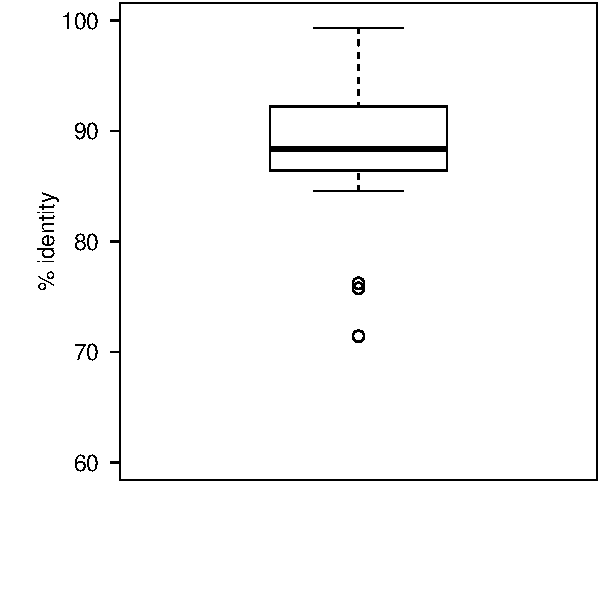
\includegraphics[width=.4\linewidth]{figure/pident_fig1} 
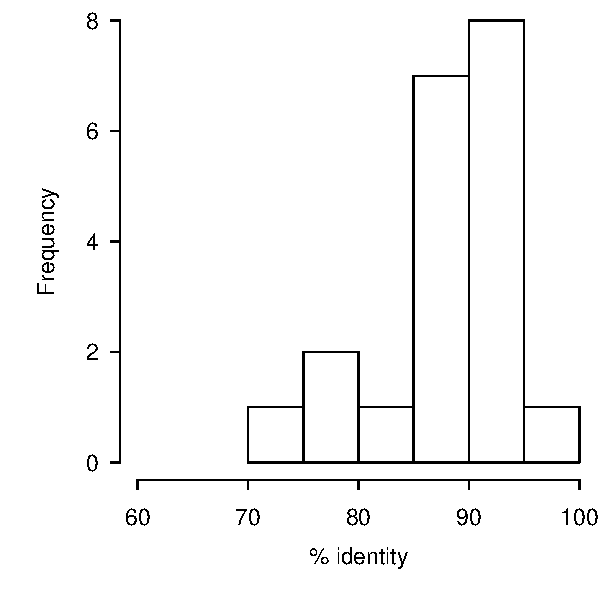
\includegraphics[width=.4\linewidth]{figure/pident_fig2} 

}



\end{knitrout}
\caption{The distribution of percent identity in the alignments of the 20 non-redundant HSP's from a default \texttt{blastn} run on the 23 query-subject pairs which resulted from the \texttt{tblastx} run (see text above).}
\end{figure}
%>>

In the folder \texttt{blast2seq\_out} I created a table called \texttt{pident.table} (see tab. \ref{pident}), which contains info about the 21 HSP's from the 23 pairwise \texttt{blastn} runs that got e-values below 0.001. Taking the average of the percent identity column of this table returns 88, meaning \textbf{my estimate of the divergence between \textit{Chorthippus} and \textit{Locusta} should be 13\%}. This divergence estimate only refers to nucleotide mismatches, not indels. Within the almost 5,000 base pairs of pairwise blast alignments, there are 23 gaps. So, there should be at least one indel (of rather small size) about every 200 bp.

The mean percent identity is 88, with a 95\% CI of (75, 101), see table \ref{blastn:comp}. The scoring scheme of the \texttt{blastn} run I did with default parameters was 2 for a match and -3 for a mismatch. Using a perl script from the Blast book \citep{Korf2003}, \texttt{example4-1.pl}, I get a target percent identity of 88.7 for this. Table \ref{blastn:comp} compares the parameters and results of two more \texttt{blastn} runs I did on the 23 \texttt{tblastx} pairs. A scoring scheme of 1, -3 looks for short alignments with almost identical sequences. The scoring scheme of 1, -1 looks for more distant matches and requires slightly longer alignments. The first (default) and the third scoring scheme do not get significant hits for the same query-subject pairs, the second scoring scheme (1, -3) misses one more pair in addition to the same pairs missed by the other \texttt{blastn} runs. Despite their very different \textsf{target \% identities}, the three \texttt{blastn} runs result in fairly similar estimates of \% identity. The second scoring scheme seems to be too stringent, so the estimate of $\sim$12--13\% divergence between the \textit{Locusta} and \textit{Chorthippus} transcriptomes seems to be robust to the match-mismatch scoring scheme used in the \texttt{blastn} runs.

There are more sophisticated methods for finding orthologous sequences from different species, which I didn't explore here. This Biostar forum thread gives a lot of information of what can be done: \url{http://www.biostars.org/p/7568/}.

%<<


\begin{figure}
\begin{knitrout}
\definecolor{shadecolor}{rgb}{0.969, 0.969, 0.969}\color{fgcolor}

{\centering 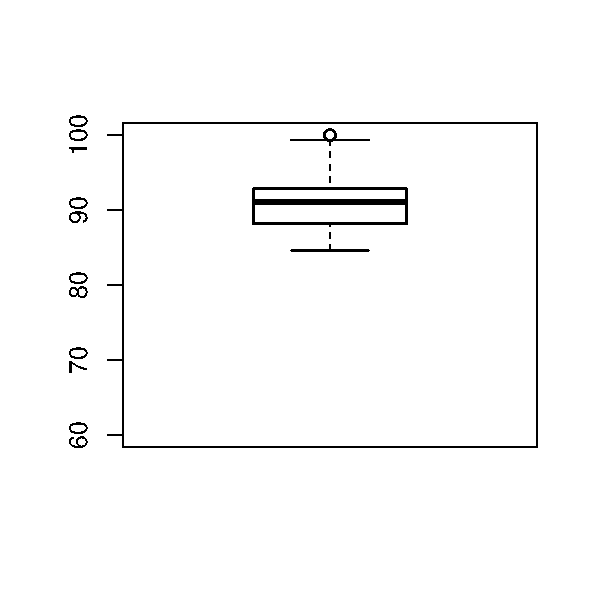
\includegraphics[width=.49\linewidth]{figure/pident_2_fig1} 
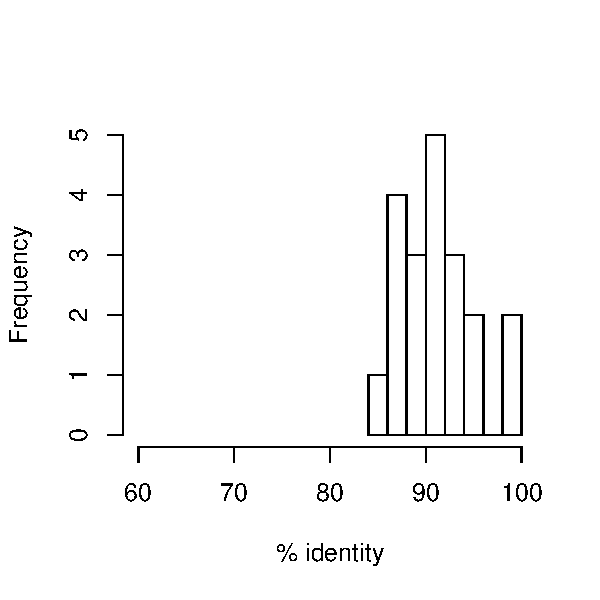
\includegraphics[width=.49\linewidth]{figure/pident_2_fig2} 

}



\end{knitrout}
\caption{Distribution of \% identity from \texttt{blastn} HSP's using a match: 1, mismatch: -3 scoring scheme.}
\end{figure}
%>>

%<<


\begin{figure}
\begin{knitrout}
\definecolor{shadecolor}{rgb}{0.969, 0.969, 0.969}\color{fgcolor}

{\centering 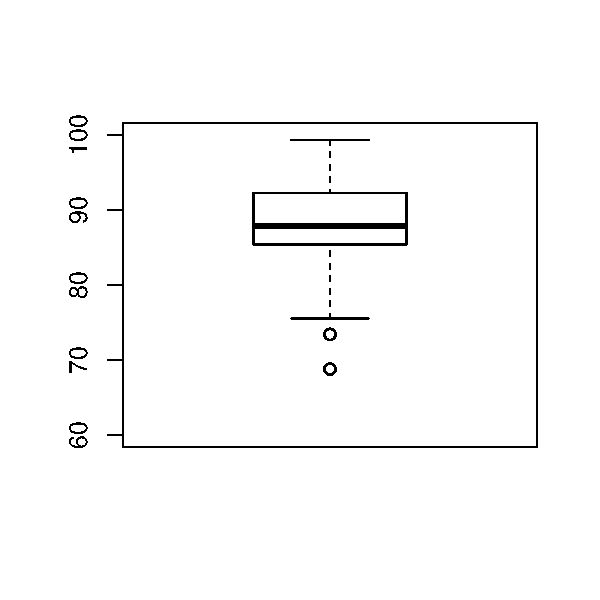
\includegraphics[width=.49\linewidth]{figure/pident_3_fig1} 
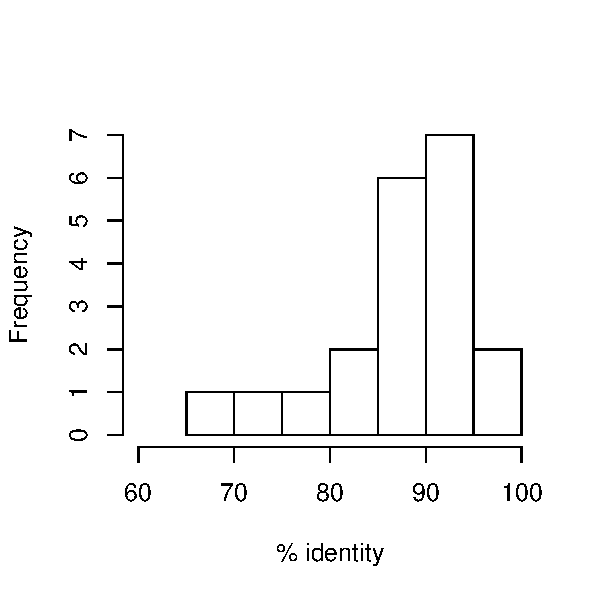
\includegraphics[width=.49\linewidth]{figure/pident_3_fig2} 

}



\end{knitrout}
\caption{Distribution of \% identity from \texttt{blastn} HSP's using a match: 1, mismatch: -1 scoring scheme.}
\end{figure}
%>>

%>> Table to compare blastn runs
\begin{table}
\caption{Comparing \texttt{blastn} runs. The \textsf{target \% identity} for each scoring scheme was determined with the \texttt{example4-1.pl} Perl script of the Blast book \citep{Korf2003}.}
\centering
%\scriptsize
%\makebox[\textwidth][c]{ % with the makebox command one can center table or figure environments on the textwidth
\begin{tabulary}{\textwidth}{ccccc} % the tabulary package with its environment tries to determine the optimal spacing of columns, which can be convenient
\toprule
\multirow{2}{*}{\textbf{match score}} & \multirow{2}{*}{\textbf{mismatch score}} & \multirow{2}{*}{\textbf{target \% identity}} & \multirow{2}{*}{\textbf{mean observed}} & \multirow{2}{*}{\textbf{95\% CI}} \\[7pt]
&&& \textbf{\% identity} & \textbf{of \% identity} \\[5pt]
\midrule
2 & -3 & 88.7 & 88 & 75, 101 \\[5pt]
1 & -3 & 98.8 & 91 & 83, 99 \\[5pt]
1 & -1 & 75 & 87 & 73, 102 \\
\bottomrule
\end{tabulary}
%}
\label{blastn:comp}
\end{table}
%>>

%%%%%%%%%%%%%%%%%%%%%%%
\subsection{Mapping of MiSeq data against \textit{Locusta} transcriptome \ldots continued}
%%%%%%%%%%%%%%%%%%%%%%%

The mapping of the "AgeI\_ery\_30-12" MiSeq reads against the Locusta unigene sequences toke 50 mins. Of the 1,226,498 AgeI\_ery\_30-12 reads 34,927 mapped with a flag of 0 (successful mapping on forward strand) and 34,911 mapped with flag 16 (successful mapping as reverse complement). \texttt{stampy} outputs those read sequences with flag 16 as reverse complement. Only about 5\% of input reads map successfully. The \texttt{stampy} mapping log file also contains the number of nucleotides that got mapped successfully, $(34,927 + 34,911) \times 96$, and the number and proportion of them that differ from the reference. \textbf{21\% of mapped nucleotides differ from the reference!}. This is a very high divergence. The posterior mapping quality scores (in the 5th column of the sam file) are relatively low, maximum of 14. Maybe that is because the actual divergence is much higher than the divergence of 0.13 that I gave \texttt{stampy} with the "--substitutionrate" switch.

The "UQ" in the \texttt{stampy} sam output file reports the read likelihood, which is the sum of phred base call qualities on mismatching sites. Note that the CIGAR string in the 6th column is not reporting matches or mismatches. \texttt{stampy} also outputs an \href{http://samtools.sourceforge.net/SAMv1.pdf}{NM} tag which gives the number of mismatches of the read to the reference. The number of mismatches are generally high, mostly between 15 and 40.

With a mapping quality score greater than 0, there are 520 \textit{Locusta} unigenes which get reads mapped to by AgeI\_ery\_30-12 and 370 unigenes with reads mapped from AgeI\_par\_34-20. 

\begin{Verbatim}
$ samtools view -F 4 AgeI_ery_30-12_sorted.bam | awk '$5>0' | cut -f3 | sort | uniq | wc -l
\end{Verbatim}

259 unigenes get reads mapped from both individuals:

\begin{Verbatim}
$ grep -cf unigenes_with_hits_from_AgeI_par_34-20 unigenes_with_hits_from_AgeI_ery_30-12
\end{Verbatim}

There are 631 Locusta unigenes which get hit by either of the two individuals.
\begin{Verbatim}
$ cat unigenes_with_hits_from_AgeI_ery_30-12 unigenes_with_hits_from_AgeI_par_34-20 \
| sort | uniq > unigenes_hit_by_either_AgeI_ind
\end{Verbatim}

Using \texttt{samtools faidx} to create an index file for the fasta file containing all Locusta unigenes (i. e. the complete reference), I can use the same samtools command to extract individual fasta sequences from the reference file by sequence name (ID). In order to extract all Locusta unigene sequences which got hits (with mapping score > 0) by either of the two individuals, I ran the following command:
\begin{Verbatim}
$ perl -ne'system("samtools faidx Locust.Unigene_short_head.fa $_") == 0 or die $!' \
unigenes_hit_by_either_AgeI_ind \
>> unigenes_hit_by_either_AgeI_ind.fa
\end{Verbatim}

\label{alignment_viewer} I have tried to browse the alignments with \texttt{samtools tview} and \texttt{tablet}. Both without success. I think this is either a bug in both programmes or the programmes are not designed to browse alignments on hundreds of reference contigs. Other people have reported the same problem on the samtools mailing list and on seqanswers, but did not get helpful answers. Fortunately, \href{http://www.broadinstitute.org/software/igv/home}{IGV} does work without any problem with my .bam files.

I want to get .bam files for each individual which
\begin{itemize}
\item only contain mapped reads 
\item with a mapping quality above 0
\item sorted by the unigene they hit
\item sorted by mapping location 
\item then by read sequence
\end{itemize}

\begin{Verbatim}
$ samtools view -F4 AgeI_ery_30-12_sorted.bam | awk '$5>0' | \
sort -k3,3 -k4,4n -k10,10 > test/AgeI_ery_30-12.test.sam
\end{Verbatim}
This skips all unmapped reads and reads with a mapping quality of 0, then sorts by unigene name, then by mapping position, then by read sequence. The resulting .sam file has no header.

\begin{Verbatim}
$ cat -S *sam | cut -f3 | uniq | tr '\n' '|' | sed 's/|$//' > pattern
\end{Verbatim}
With this command I am taking the unigene names that got hits by AgeI\_ery\_30-12 and create a regular expression pattern out of them.

\begin{Verbatim}
$ perl -ne'BEGIN{$p=`cat pattern`; chomp $p;} if(/^\@SQ/){print if /$p/o;}else{print}' header \
> header_reduced
\end{Verbatim}
With this command I am first reading in the pattern. Then I am going over each line in the header file taken from the original .bam containing all 12,641 unigene names in the header. Lines starting with "@SQ" contain the unigene names (usually chromosome or contig names). They are only printed out if they contain a unigene name that got hit by AgeI\_ery\_30-12. I also have to sort the unigene names in the header, which I do with the following command:
\begin{Verbatim}
$ tr ':' '\t' < header_reduced_without_HD_PG_CO \
| sort -k 3,3 | sed 's/N\t/N:/g' \
> header_reduced_without_HD_PG_CO_sorted
\end{Verbatim}
This takes the new header file which only contains names of unigene which got hit and I also removed the first three lines, which contain additional info. The transliterate command turns a colon into a tab character, so that unigene names are in their own column (this is probably not necessary, but better be safe). I then sort the file by the unigene names and revert it back into the old format. Putting it all back together again:
\begin{Verbatim}
$ cat HD_PG_CO header_reduced_without_HD_PG_CO_sorted AgeI_ery_30-12.test.sam \
> AgeI_ery_30-12_sorted.sam
$ samtools view -bS AgeI_ery_30-12_sorted.sam > AgeI_ery_30-12_sorted.bam
$ samtools index AgeI_ery_30-12_sorted.bam
\end{Verbatim}

6.9\% of all EagI\_ery\_30-12 and 7\% of all EagI\_par\_34-20 reads map to the Locusta transcriptome. With a mapping quality of above 0, there are 352 Locusta unigenes that get hit by EagI\_par\_34-20  and 462 that get hit by EagI\_ery\_30-12 reads. There are 212 Locusta unigenes that get hit by both EagI individuals with a mapping quality of above 0.
\begin{Verbatim}
$ cat unigenes_hit_by_EagI_ery_30-12 unigenes_hit_by_EagI_par_34-20 | sort | uniq | wc -l
\end{Verbatim}
There are 602 unigenes that got hit by either EagI individual. I order to produce a reduced reference sequence, which only contains unigene sequences which got hit by either EagI individual, I used the \texttt{samtools faidx} command.
\begin{command}
\captionsetup{type=command}
\begin{Verbatim}
$ perl -ne'system("samtools faidx Locust.Unigene_short_head.fa $_") == 0 or die $!' \
unigenes_hit_by_either_EagI_ind \
>> unigenes_hit_by_either_EagI_ind.fa
\end{Verbatim}
\caption{Example of a command line that extracts fasta sequences from an indexed multi-fasta file using a file listing fasta headers.}
\label{reduced_reference}
\end{command}
I then load this reduced reference sequence into IGV together with the sorted and indexed .bam file of each individual.

The first thing that is conspicuous is how rarely mapped reads from both sides of the SbfI restriction site can be found. However, with a double-digest library this is expected! In fact, in order to get reads from both sides of the restriction site, there would need to be an AgeI (or EagI, depending on the library) restriction site within a few hundred base pairs on either side of the SbfI restriction site. There are, however, several cases where reads map to both sides of an SbfI restriction site (tab. \ref{both_sides_tab} and fig. \ref{both_sides_fig}). PCR primers could be designed for them in order to test complete digestion with SbfI via qPCR. The PCR products would only be around 180bp long. The first RAD library I sequenced was a standard RAD library. With this library there should be many SbfI restriction sites where reads from both sides get mapped and possibly also their paired-end reads, allowing for longer PCR products. 

\begin{table}[b]
\centering
\caption{a non-complete list of Locusta unigenes to which SbfI-AgeI RAD reads map to both sides of the SbfI site.}
\begin{tabular}{c}
\toprule
unigene names\\
\midrule
LMC\_000661\\
LMS\_004974\\
LMS\_007593\\
LMS\_005092\\
LMS\_001256\\
LMS\_001110\\
\bottomrule
\end{tabular}
\label{both_sides_tab}
\end{table}

\begin{figure}
\centering
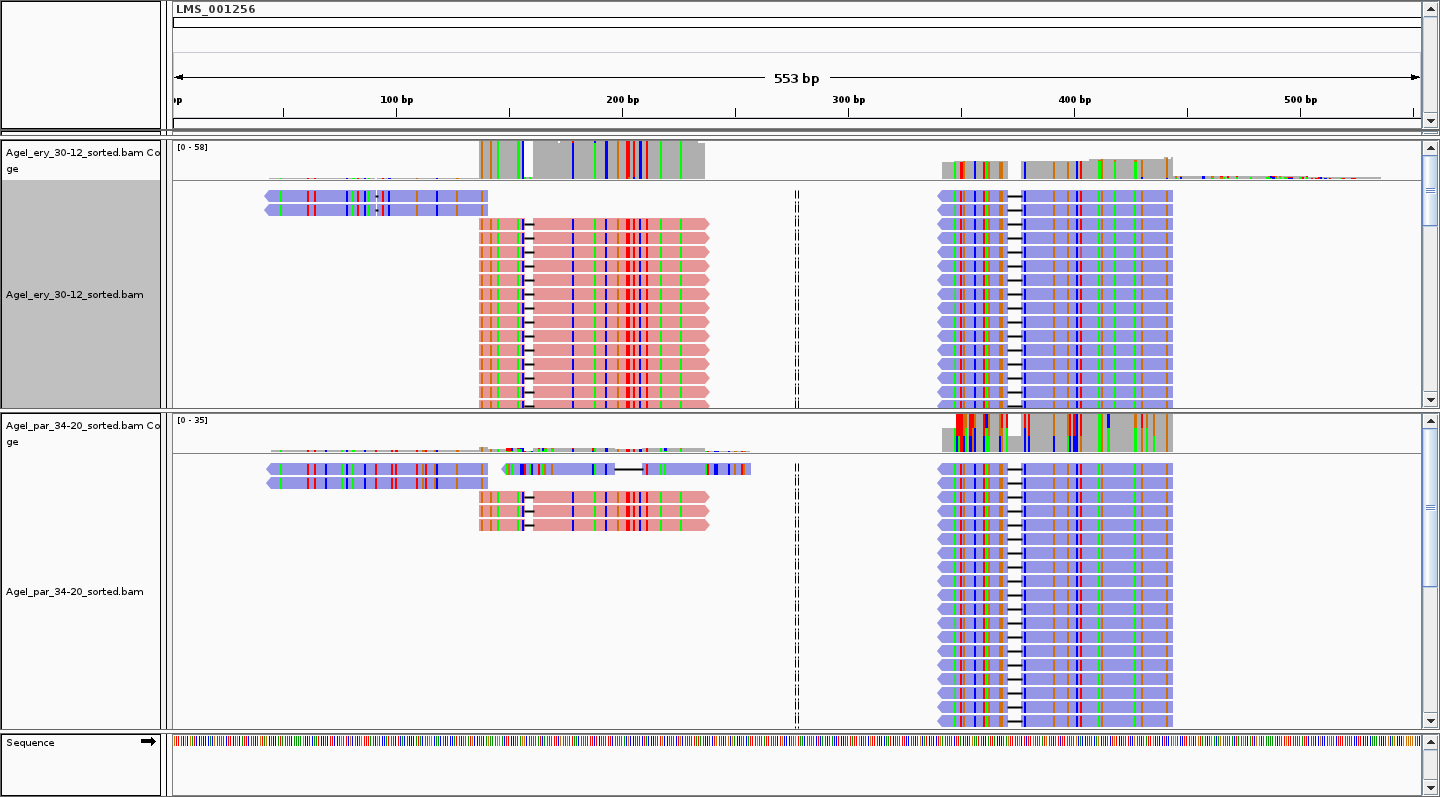
\includegraphics[width=\textwidth]{./figure/igv_LMS_001256}
\caption{Alignment of SbfI-AgeI reads to the Locusta unigene LMS\_001256 viewed in \texttt{IGV}. The left half shows alignments of reads to both sides of an SbfI restriction site.}
\label{both_sides_fig}
\end{figure}

The alignments of both MiSeq libraries are generally wild and often very divergent reads get mapped to the same location in the reference (fig. \ref{igv_LMC_003278}). 

\begin{figure}
\centering
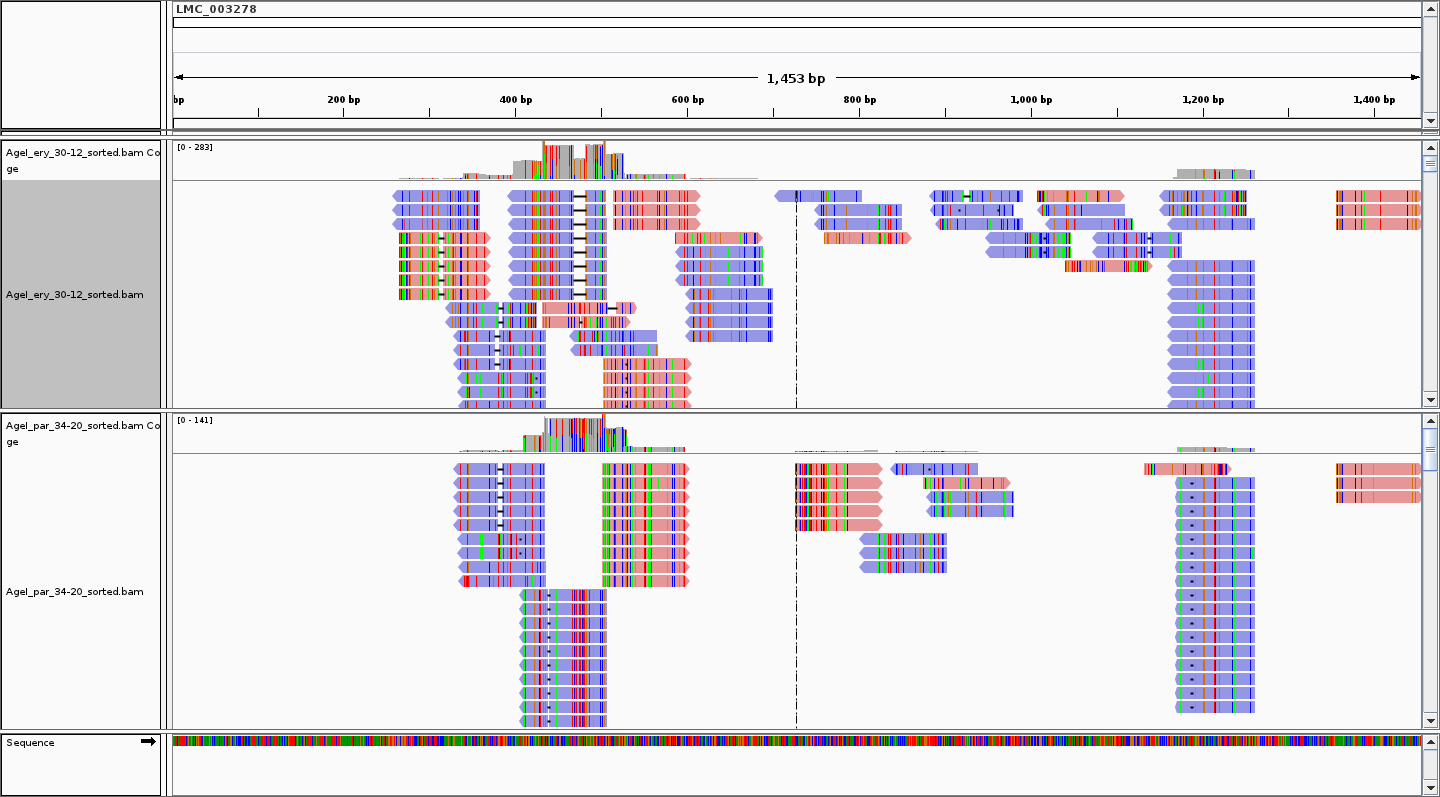
\includegraphics[width=\textwidth]{./figure/igv_LMC_003278}
\caption{Alignments of SbfI-AgeI reads to the Locusta unigene LMC\_003278. Most alignments also show, among well aligned reads, very divergent \textit{Chorthippus} reads aligned to overlapping positions.}
\label{igv_LMC_003278}
\end{figure}

I don't think it is worth spending time on trying to call SNP's with these alignments, although rare exceptions do exist (fig. \ref{igv_LMC_001848}). Given the small percentage of reads that map, I also don't deem it worth only using those successfully mapping reads as input for a de-novo assembly. Even if the reference contigs from such an assembly were more reliable than those created from all RAD reads (because expressed sequences supposedly are less repetitive), they would provide a reference for less than 10\% of reads. 

\begin{figure}
\centering
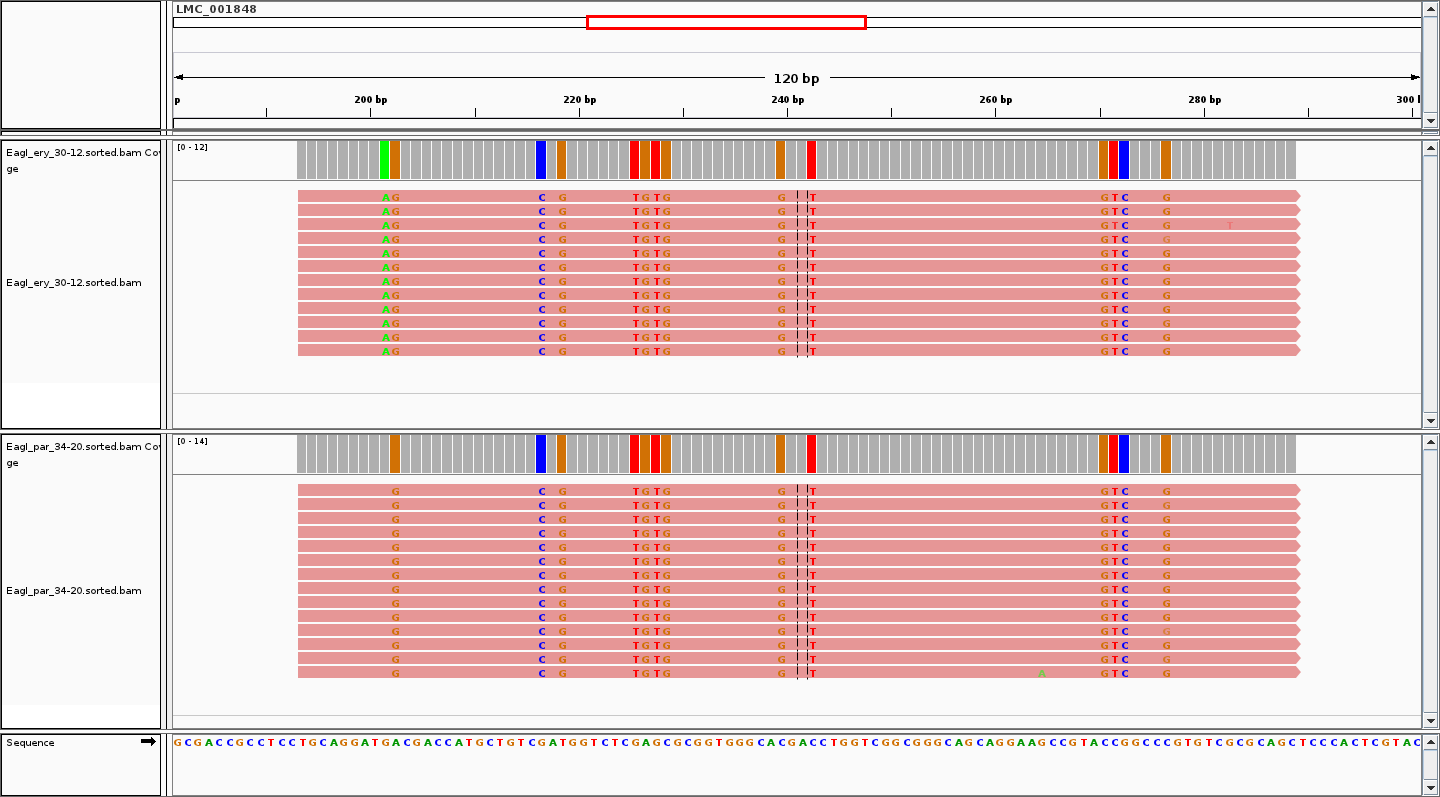
\includegraphics[width=\textwidth]{./figure/igv_LMC_001848}
\caption{Clear A/G SNP in SbfI-EagI RAD tag between the individual ery\_30-12 and par\_34-20 at unigene LMC\_001848}
\label{igv_LMC_001848}
\end{figure}

\begin{figure}
\centering
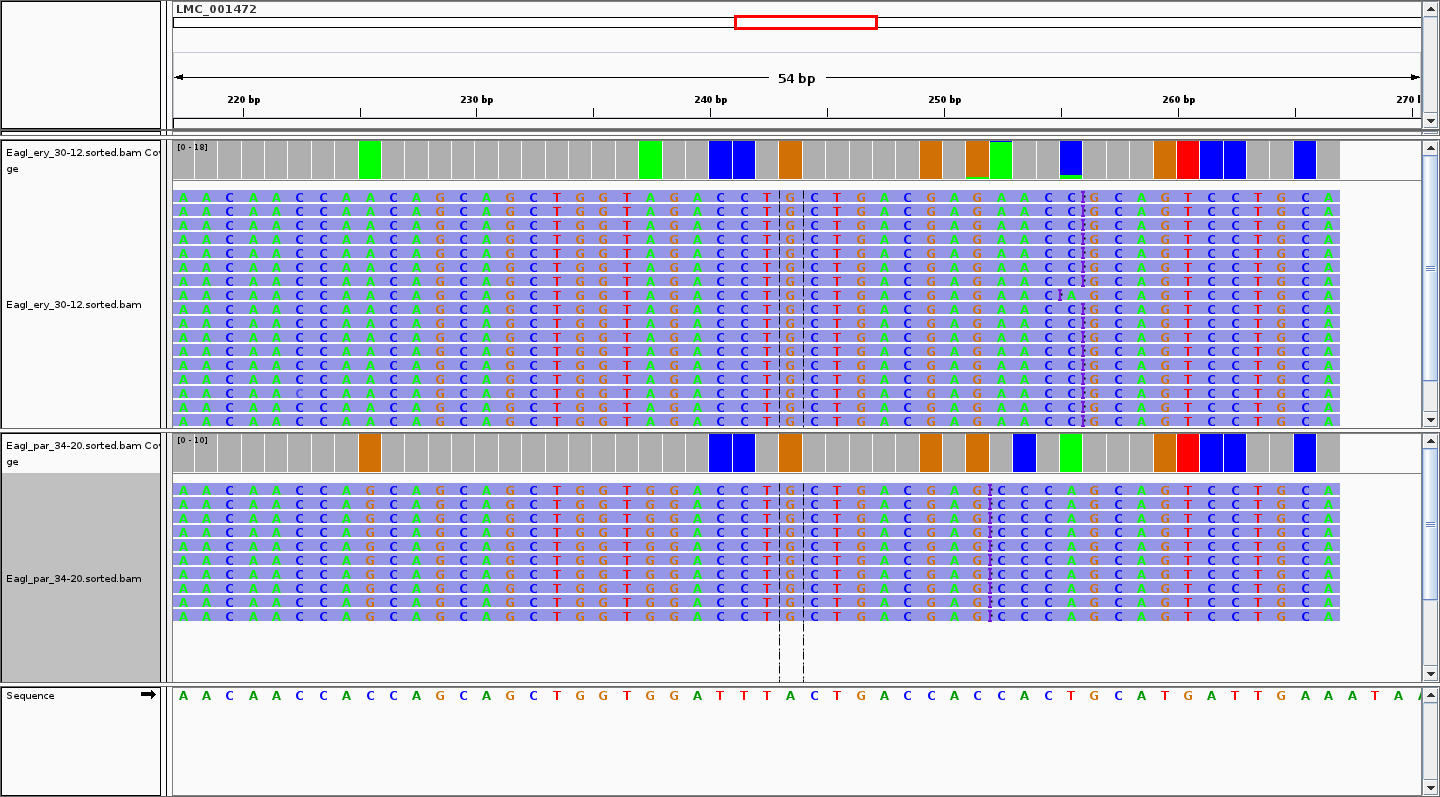
\includegraphics[width=\textwidth]{./figure/igv_LMC_001472}
\caption{An SbfI-EagI RAD tag hitting Locusta unigene LMC\_001472 shows 4 divergent SNP's between the ery\_30-12  and the par\_34-20 individual. One SNP is concealed in the alignment due to the placement of a 2 base pair insertion at different positions in the two individuals.}
\label{igv_LMC_001472}
\end{figure}

A \texttt{Muscle} alignment in clustalw output format of SbfI-EagI reads hitting Locusta unigene LMC\_001472 is shown in fig. \ref{muscle_LMC_001472}. Both individuals show a 2 base pair insertion with respect to the \textit{Locusta} reference, which stampy had placed at different positions in the two individuals.

\begin{figure}
\centering
\begin{Verbatim}
ery_30-12               CCATCACCAAGTGGGGGCAGACGCCGCTAGACATCGCCAGGGGCAACAACCAACAGCAGC
par_34-20               CCATCACCAAGTGGGGGCAGACGCCGCTAGACATCGCCAGGGGGAACAACCAGCAGCAGC
                        ******************************************* ******** *******

ery_30-12               TGGTAGACCTGCTGACGAGAACCCAGCAGTCCTGCA
par_34-20               TGGTGGACCTGCTGACGAGAGCCCAGCAGTCCTGCA
                        **** *************** ***************
\end{Verbatim}
\caption{Alignment of the consensus sequences of the two individuals at locus LMC\_001472 (see fig. \ref{igv_LMC_001472}) revealing a hidden SNP due to different placement of an insertion in the two alignments. Multiple sequence alignment of the reads of both individuals would place the gap consistently and reveal all 4 SNP's. It is possible that the \texttt{samtools mpileup} command could deal with this.}
\label{muscle_LMC_001472}
\end{figure}

%%%%%%%%%%%%%%%%%%%%%%%
\subsection{Amy's highly significant locus \texttt{4C-A12}}
\label{4C-A12}
%%%%%%%%%%%%%%%%%%%%%%%
Note, 4C-A12 is not the only locus showing strong expression differences and SNP differences between the two subspecies.

4C-A12 matches a single Locusta unigene, LMS\_002733, in a default \texttt{tblastx} with an e-value of 3e-29. However, these local alignments are not from translations within the reading frames of the longest ORF's that can be found in both sequences. They are most likely based on non-coding DNA sequence conservation. This \textit{Locusta} EST cluster is 686bp long. Its longest ORF is 86 aa long and on the 6th reading frame (from the output of \texttt{translation.pl} on  \texttt{Locusta\_single\_hit.fasta}). If this was a real ORF, then 62\% of that transcript would be UTR, which I think is unusual at least. The translations of the longest ORF's of each sequence do not show any similarity.

Ms Badisco and Mr Vanden Broek have kindly sent me the \texttt{Phrap} assembled \textit{Schistocerca} transcriptome and \texttt{Blast2GO} annotation of it. The assembled transcriptome is in the file called \texttt{LC\_unique.seq}, which contains 12,709 sequences and is 10,849,701 bp long in total. I created a window- and dust masked blast database from this file and used \texttt{blastn} to query this database with the 4C-A12 sequence from \textit{Chorthippus}. I get one highly significant HSP with a \textit{Schistocerca} sequence that doesn't seem to have been clustered: LC03019B1F08.f1. This Schisto EST is 772 bp long and in lower case in the LC\_unique.seq file, indicating that a filtering programme has found this to be a repetitive sequence. Window- and Dustmasker mask only part of that sequence. \cite{Badisco2011} used \href{http://www.repeatmasker.org/}{RepeatMasker} to mask EST's before the assembly.

I used \href{http://www.girinst.org/censor/index.php}{\textsf{RepBase}}'s web search interface (see fig \ref{censor}) to search the repeat database with the 4C-A12 from \textit{Chorthippus} and the two homolog sequences from \textit{Locusta} and \textit{Schistocerca}. The \textit{Chorthippus} sequence does not get a hit, but the the two other sequences do:
\begin{itemize}
\item the \textit{Locusta} sequence hits a DNA transposon from \textit{Drosophila ficusphila} with an alignment length of 81 bp
\item the \textit{Schistocerca} sequence hits a 35 bp fragment of a DNA transposon from \textit{Acyrthosiphon pisum}
\end{itemize}
So there is tentative support for an annotation of 4C-A12 as a highly derived DNA transposon or rather a relict of it, given that the only short alignments are outside of ORF's for transposase. I have saved the \texttt{CENSOR} output as well alignment files on huluvu in \texttt{/data/claudius/Read\_mapping/4C-A12} .

\begin{figure}
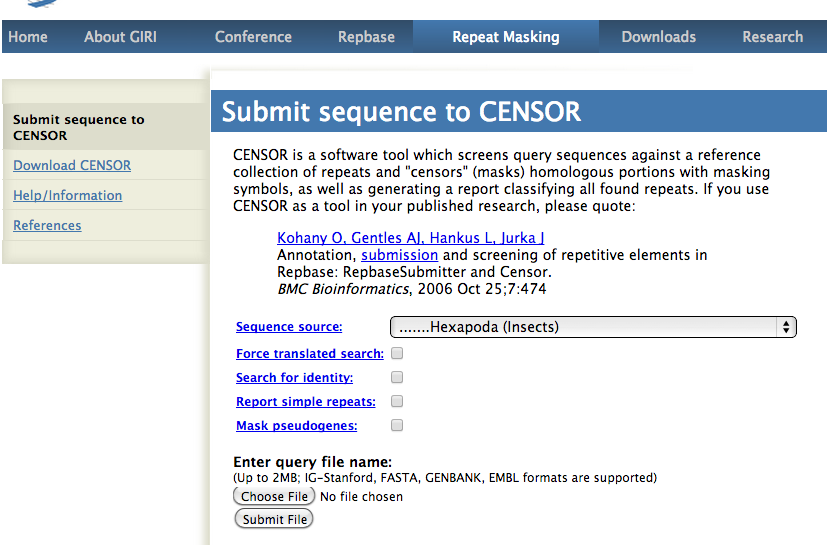
\includegraphics[width=.9\textwidth]{./figure/CENSOR}
\caption{The web interface to the RepBase.}
\label{censor}
\end{figure}


%%%%%%%%%%%%%%%%%
\subsection{\textit{Schistocerca}}
%%%%%%%%%%%%%%%%%

This only contains Poly(A)-transcripts, from the central nervous system \citep{Badisco2011}. The cDNA was normalised (Evrogen) before Sanger sequencing. Repeat and low complexity sequences were identified and masked by using \textsf{RepeatMasker}. E. coli, vector, mitochondrial, ribosomal and viral DNA was detected with \textsf{blastn} and removed. Ds cDNA was size selected for fragments longer than 600 bp. Assembly of sequences into contigs was performed by using the \texttt{Phrap} software package. When transcripts were represented by only one sequence, the EST was referred to as a 'singleton'.

I downloaded all 34,672 raw \textit{Schistocerca} EST's from \href{http://www.ncbi.nlm.nih.gov/nucest}{Genbank}, using the following search details:
\verb! ("Schistocerca"[Organism] OR schistocerca[All Fields]) AND "Schistocerca gregaria"[porgn] ! \\

I downloaded all sequences using the \textsf{Send to} button at the online interface to the Genbank EST database (fig. \ref{SendTo}).
However, I also have the \texttt{Phrap} assembled Schistocerca transcriptome from Badisco and vanden Broek (see section \ref{4C-A12}).

\begin{figure}
\centering
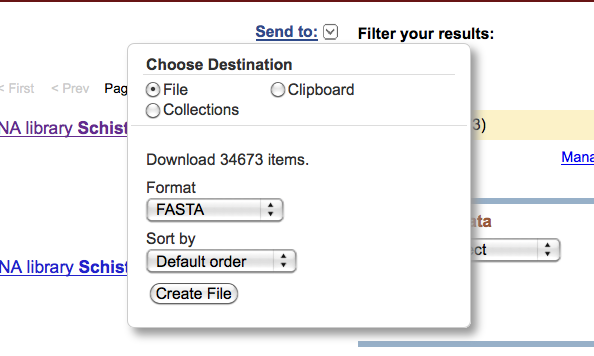
\includegraphics[width=.8\textwidth]{./figure/Schistocerca-EST-download}
\caption{Via "Send To > File", all 34,673 sequences can be downloaded.}
\label{SendTo}
\end{figure}

I used the \textit{Schisto} Phrap assembled transciptome as a reference for stampy mapping specifying again a substitution rate of 0.13. The stampy log files report again that 20\% of mapped nucleotides differ from the reference for both double digest libraries. The \textit{Schisto} transcriptome contains 12,709 contigs.

I created sorted bam files that only contain mapped reads with a mapping quality of > 0 (i. e. unambiguous mapping position) with the following command line:
\begin{command}
\captionsetup{type=command}
\caption{Example of a command that extracts mapped reads with mapping quality above 0 and creates a position sorted .bam file.}
\begin{Verbatim}
$ samtools view -hSF4 AgeI_ery_30-12.sam.gz | \
awk '{if(/^\@/){print}else{if($5>0){print}}}' | samtools view -uhS - | \
samtools sort - AgeI_ery_30-12_sorted
\end{Verbatim}
\label{filter_good_reads}
\end{command}

\begin{table}
\centering
\caption{Proportion of successfully mapped reads against the \textit{Schistocerca} transcriptome with mapping quality > 0.}
\begin{tabular}{lr@{.}lccc}
\toprule
individual & \multicolumn{2}{c}{mapped reads}  & \# of contigs hit & contigs hit by both ind. & contigs hit by either ind.\\
\midrule
AgeI\_ery\_30-12 & \qquad 10&6\% & 723 & \multirow{2}*{326} & \multirow{2}*{864}\\
AgeI\_par\_34-20 & 11&0\% & 503\\
\midrule
EagI\_ery\_30-12 & 12&1\% & 604 & \multirow{2}*{316} & \multirow{2}*{753}\\
EagI\_par\_34-20 & 12&2\% & 465\\
\bottomrule
\end{tabular}
\end{table}

\begin{figure}
\centering
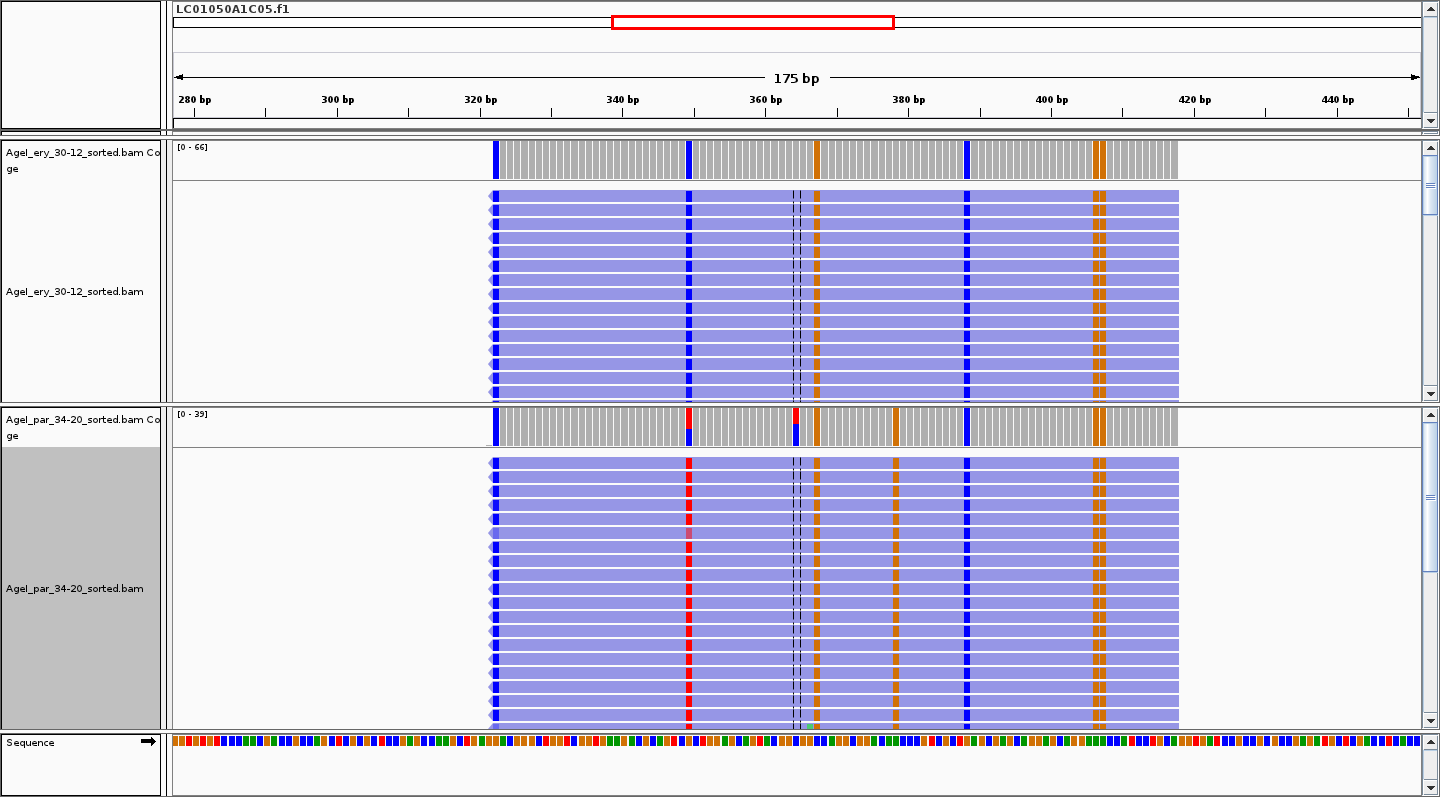
\includegraphics[width=\textwidth]{./figure/igv_LC01050A1C05}
\caption{At the \textit{Schistocerca} contig LC01050A1C05.f1 the AgeI\_par\_34-20 individual (bottom) is heterozygous for two SNP's. The two haplotypes in this individual have read count proportions 44\% and 56\% with a total read count of 39.}
\label{igv_LC01050A1C05.f1}
\end{figure}

\begin{figure}
\centering
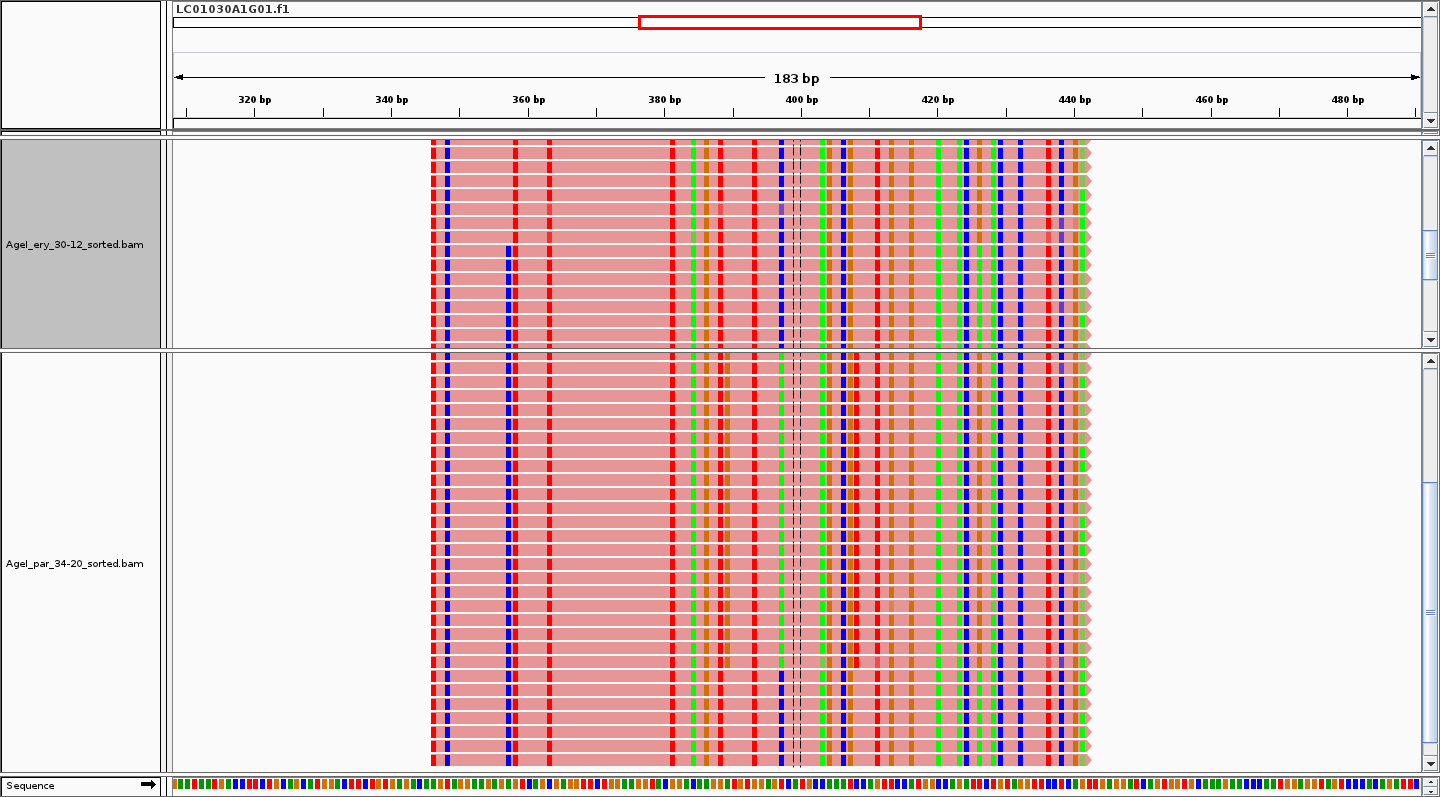
\includegraphics[width=\textwidth]{./figure/igv_LC01030A1G01}
\caption{At the \textit{Schistocerca} contig LC01030A1G01, AgeI\_ery\_30-12 (top) has almost even coverage for its two haplotypes (55\% to 45\%) at a total read count of 47. In contrast, AgeI\_par\_34-20 (bottom) has coverage 18\% to 82\% for its two haplotypes at a total read count of 39.}
\label{}
\end{figure}

\pagebreak


%%%%%%%%%%%%%%%%%%%%%%%%%%%%%%%%%%%%%%%%
\section{Mapping of MiSeq reads against the \textit{Timema} reference genome}
%%%%%%%%%%%%%%%%%%%%%%%%%%%%%%%%%%%%%%%%

\textit{Timema} is not an orthopteran insect. The species complex is currently grouped with other stick insects at the base of the order \textit{Phasmida}. Based on morphological data, the orders \textit{Orthoptera} and \textit{Phasmida} are sister groups (see \href{http://tolweb.org/Neoptera/8267}{Tree of Life} homepage).

I have mapped the MiSeq reads against the \textit{Timema} genome reference called \emph{allpaths-assem-11nov12.lg}  kindly provided by Victor. Excluding N's used to separate contigs within scaffolds, the \textit{Timema} reference is 843,259,983 bases long.

I have given \texttt{stampy} an expected substitution rate of 20\% this time. The parallel mapping of the 4 MiSeq files took 1 hour and 22 minutes. \texttt{stampy} reports that between 22\% and 26\% of mapped nucleotides differ from the reference. The mapping quality scores range only from 0 to 4. I don't understand why they are so low. Maybe this is due to the much bigger reference sequence as compared to the transcriptomes, which allows for more alternative mapping positions.

I created sorted bam files only containing mapped reads with a quality score above 0 slightly differently as before: using the "-q" switch of the \texttt{samtools view} command to filter out reads mapped with ambiguous position instead of using an \texttt{awk} command for this. That change allowed me to parallelise this task:
\begin{command}
\captionsetup{type=command}
\caption{Convert .sam files into postion sorted bam files in parallel filtering out unmapped reads and reads with mapping quality below 1}
\begin{Verbatim}
$ ls *sam.gz | parallel 'samtools view -hSF4 -q1 {} | \
samtools view -uhS - | samtools sort - {.}_sorted' &
\end{Verbatim}
\label{convert_sam_to_bam}
\end{command}
Only between 1,274 and 6,700 \textit{Chorthippus} reads get mapped to the \textit{Timema} reference, i. e. $\le$ 0.5\% of all input reads.

In figure \ref{igv_lgNA_ordNA_scaf6182} the individual AgeI\_ery\_30-12 has reads mapped to both sides of the SbfI restriction site. While one side got more than 100 reads the other got only two. The other individual AgeI\_par\_34-20 did not get any reads from this locus. I think this pattern cannot be explained simply by random uneven coverage. Polymorphisms in the SbfI and/or AgeI restriction sites could explain this. However, this seems quite unlikely given the relatively low divergence towards the \textit{Timema} reference indicating a rather low substitution rate at this locus.

\begin{figure}[hbp]
\centering
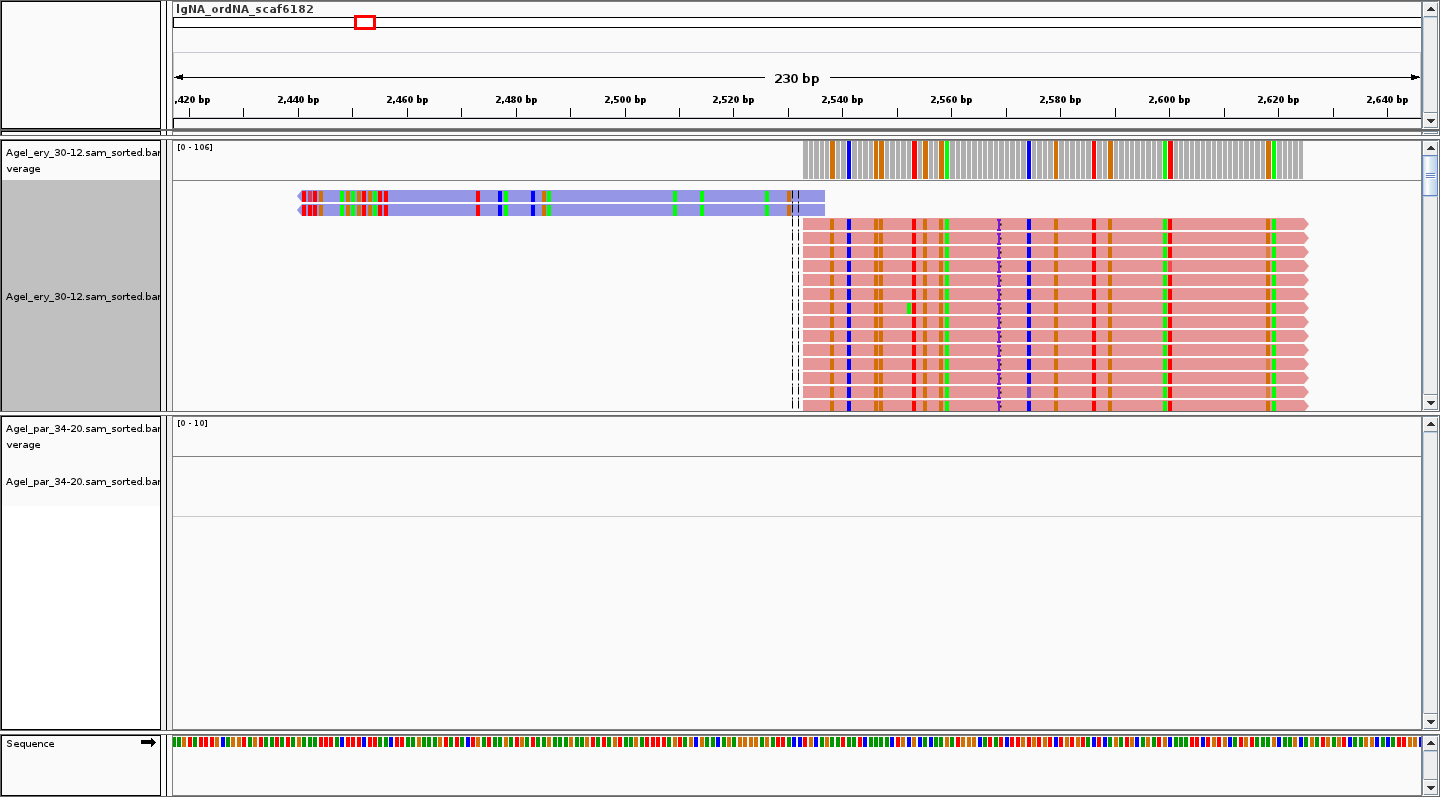
\includegraphics[width=\textwidth]{./figure/igv_lgNA_ordNA_scaf6182}
\caption{Example of reads mapped to \textit{Timema} scaffold lgNA\_ordNA\_scaf6182 at position 2,417-2,645. }
\label{igv_lgNA_ordNA_scaf6182}
\end{figure}

In figure \ref{igv_lg4_ord135_scaf170} the upper individual gets 166 reads, the lower 73. The upper individual got about twice as many reads in total from the sequencing run as the lower individual. So this can explain the difference in coverage at this locus. Also, the heterozygous SNP in the upper individual has allele coverage 45\% to 55\%. Taken together with observations from alignments to the transcriptomes, this indicates to me that  PCR drift generally has not caused uneven allele coverage and, hence, if strong allele bias is observed, other causes must be assumed, e. g. alignment of paralogous sequences together with allele-drop-out (due to polymorphism in the restriction site) at one of the two copies.

\begin{figure}
\centering
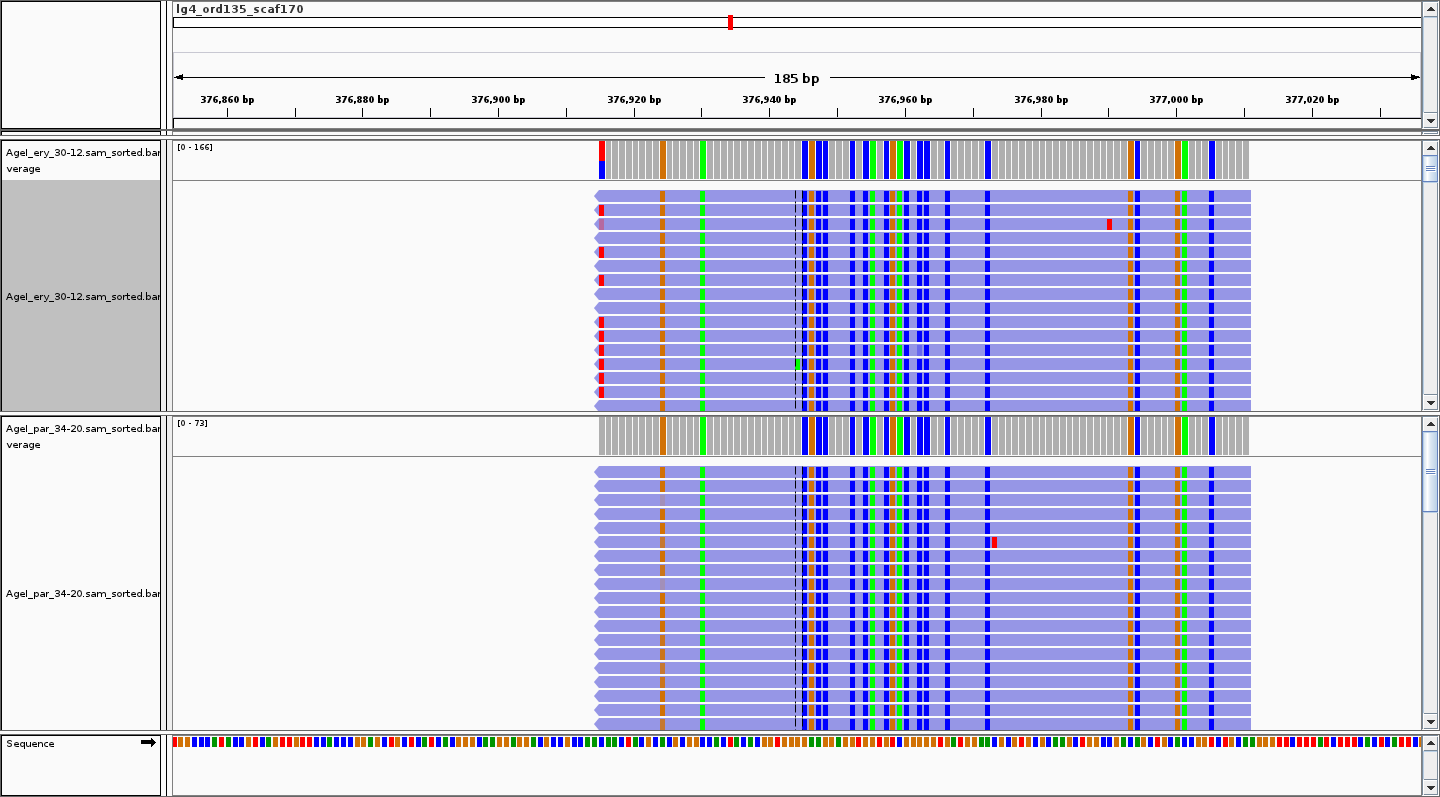
\includegraphics[width=\textwidth]{./figure/igv_lg4_ord135_scaf170}
\caption{Example of reads mapped to \textit{Timema} scaffold lg4\_ord135\_scaf170 at position 376,852. See text for explanation.}
\label{igv_lg4_ord135_scaf170}
\end{figure}


%%%%%%%%%%%%%%%%%%%%%%%%%%%%%%%%%%%%%%%%
\section{Mapping of the "Big Data" standard RAD paired reads}
%%%%%%%%%%%%%%%%%%%%%%%%%%%%%%%%%%%%%%%%

\subsection{\textit{Schistocerca}}

\roger{I first try to map the \texttt{process\_radtags} purified reads from one individual of each subspecies against the \textit{Schistocerca} reference. I am using the reads from \texttt{ery\_30-12} (1,227,495) and \texttt{par\_34-10} (975,810).} These reads still contain adapter sequences, but the adapter contamination in these reads is much lower than in the libraries sequenced on MiSeq (on the order of 0.1-0.2\%, see command \ref{adapter_fuzzy_grep}). In contrast to de novo assemblies (see Kang-Wook's adapter screening script), reads into adapter should not interfere with independent mapping of reads. Reads into adapters will simply not map or with many mismatches. If they do map, they might interfere with SNP calling, though.

\begin{command}
\captionsetup{type=command} % this is necessary for the hyperlink to work, see manual for caption package, 6.5 about hyperref
\begin{Verbatim}
$ zcat ery_30-10.fq_1.gz | awk '(NR-2)%4==0' | tre-agrep -1 AGATCGGAAG | wc -l
\end{Verbatim}
\caption{Searching reads for the first 10 bp's of adapter sequence with 1 bp fuzzy matching}
\label{adapter_fuzzy_grep}
\end{command}

I used command \ref{qual_format} to check whether the reads in the Big Data set came with Phred+33 formatted quality strings. They did not. All reads in the Big Data set (4 GAIIx lanes) came with Phred+64 formatted quality strings. So, a base call quality score of 0 is encoded by "@". \roger{The single-end reads are 46 bp long (after removal of barcode sequence) and the paired-end reads are 51 bp long.} The running time logging didn't work this time, but \texttt{stampy} took more than one hour to finish mapping the reads of both individuals. \roger{I ran \texttt{stampy} with a substitution rate of 13\% again.} Strangely, the \texttt{stampy} log files report that only about 3\% of nucleotides are different from the reference. This is based on 96\% of input reads. This does not make sense. I also specified a mean insert size of 400 bp and an insert size standard deviation of 100 bp. \texttt{stampy}'s estimate of the mean insert size is $\sim$100 bp only for both individuals with a standard deviation of only 34 bp, which for both individuals is based on $\sim$300,000 read pairs (see stampy log files). However, according to the reported SAM flags, there are only 47,240 read pairs from individual \texttt{ery\_30-12} where both reads got mapped, even if in improper pairs. The README file of \texttt{stampy} explains some of its output (section 10.2 SAM output format):
\begin{quote}
\textsf{
The "proper pair" flag bit (value 2) is set if two reads are correctly oriented, and their separation is within 5 standard deviations from the mean.
}
\end{quote}
So, it is not clear which read pairs \texttt{stampy} used to empirically determine the distribution of insert sizes. It is anyway not very surprising that the empirical insert size is much lower than expected from the size range extracted from the gel (minus the combined length of illumina adapters), i. e. $\sim$ 300-600 bp, since firstly PCR and illumina sequencing increase the proportion of small insert size fragments and secondly the mapping against a transcriptome means that often one mate of a read pair either maps on another contig/unigene or doesn't map at all and small insert size fragments are more likely to have both of their reads mapped to the same contig.

\begin{table}
\caption{\texttt{samtools view -X} prints a single letter or number for each bit set in the flag for a read in the SAM file.}
\centering
\begin{tabular}{cl}
\toprule
code & meaning \\
\midrule
p & read is paired in sequencing \\
P & read and its mate have been properly mapped \\
u & read is unmapped \\
U & mate is unmapped \\
r & read printed as reverse complement of input \\
R & mate printed as reverse complement of input \\
1 & read is first in pair \\
2 & read is second in pair \\
\bottomrule
\end{tabular}
\label{samtools_view_X}
\end{table}

I have written a little perl script \texttt{SAMflag.pl} which takes a .sam or .bam file and counts the number of reads for each SAM flag as well as reporting the meaning of the bits set in each flag. This way the horribly cryptic SAM flags become a bit more verbose. A totally undocumented alternative is the (hidden) "-X" switch to the \texttt{samtools view} command which replaces the integer flag in the SAM file with a code that indicates which bits have been set (see table \ref{samtools_view_X}). The flag integers 99, 147, 83 and 163 indicate that the read has been mapped in a proper pair (i. e. with inverse orientation of read pairs and an insert size within 5 sd of mean). For instance, the flag integer 99 is decimal for 11000110: the 0th bit is set $\rightarrow$ read is from paired-end sequencing; the 1st bit is set $\rightarrow$ read is mapped in a proper pair; the 5th bit is set $\rightarrow$ mate is printed as reverse complement of input; the 6th bit is set $\rightarrow$ read is first in pair (see table \ref{SAM_flag_bits}). Obviously, 99 is the sum of the bit values set.

\begin{table}
\centering
\caption{SAM flag bits and their meaning taken from the \href{http://picard.sourceforge.net/explain-flags.html}{picard site}.}
\begin{tabular}{crl}
\toprule
bit & value & meaning \\
\midrule
0 & 1 & read is from paired-end sequencing \\
1 & 2 & read is mapped in a proper pair \\
2 & 4 & read is unmapped \\
3 & 8 & mate is unmapped \\
4 & 16 & read is printed as reverse complement of input \\
5 & 32 & mate is printed as reverse complement of input \\
6 & 64 & read is first in pair \\
7 & 128 & read is second in pair \\
\bottomrule
\label{SAM_flag_bits}
\end{tabular}
\end{table}

This \href{http://picard.sourceforge.net/explain-flags.html}{picard site} explains the meaning of the 0th to 11th bit (from top to bottom) that can be set in the SAM flags and combinations thereof. Figure \ref{sam_flags_meaning} gives further clarification about the meaning of SAM flags.

\begin{figure}[htp]
\centering
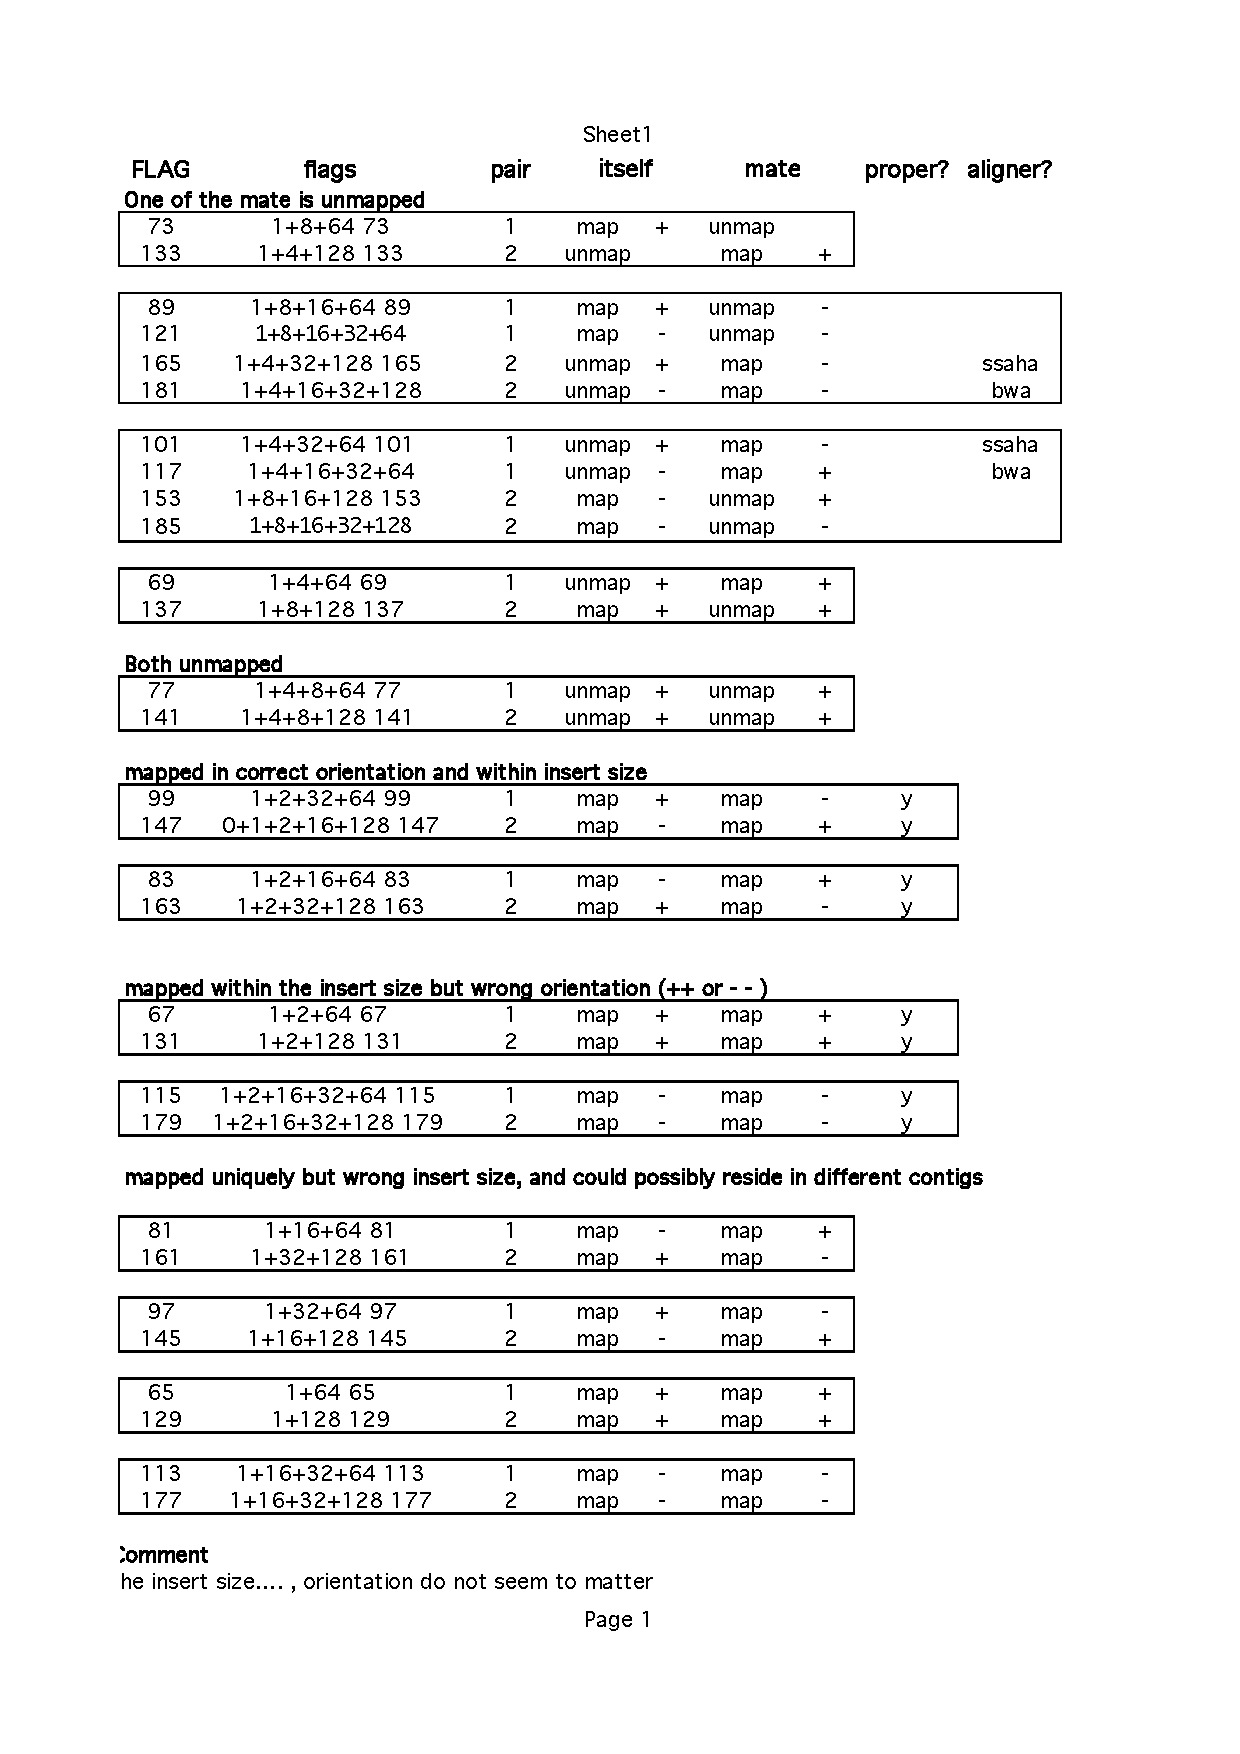
\includegraphics[height=.9\textheight]{./figure/sam_flags_meaning}
\caption{The meaning of SAM flags explained. Taken from \href{http://ppotato.wordpress.com/2010/08/25/samtool-bitwise-flag-paired-reads/}{this} website. Note that for the reads "mapped within the insert size but with wrong orientation" \texttt{stampy} would not set the bit value 2 for "proper" mapping.}
\label{sam_flags_meaning}
\end{figure}

In addition to properly mapped read pairs, I am also interested in looking at those pairs where both reads got mapped, even if not in the expected inverse orientation or with an insert size that is within 5 (empirical) standard deviations of the mean. With the "-F" switch to the \texttt{samtools view} command I can skip reads where either read in a pair has not been mapped. Those reads will either have the bit value 4 or 8 set. Command \ref{filter_unmapped_read_pairs} gets rid of read pairs where either read is unmapped. Note, that the two versions in command \ref{filter_unmapped_read_pairs} are equivalent.

\begin{command}
\captionsetup{type=command} % this is necessary for the hyperlink to work, see manual for caption package, 6.5 about hyperref
\begin{Verbatim}
$ samtools view -F 12 -S ery_30-12.sam.gz
$ samtools view -S ery_30-12.sam.gz | awk 'and($2, 12)==0'
\end{Verbatim}
\caption{Command line that extracts all read pairs where both reads in a pair got mapped (properly or not).}
\label{filter_unmapped_read_pairs}
\end{command}

\texttt{stampy}'s README file explains what mapping quality is assigned to reads or read pairs with ambiguous mapping locations. In section \textrm{11.5 Multiple mapping locations} it says:
\begin{quote}
\textsf{
Normally, when Stampy identifies several equally good mapping locations for a read or read pair, it reports one of these at random (and assigns the choice a low mapping quality, of 3 or less).
}
\end{quote}
\textbf{So anything with a mapping quality below 4 is ambiguous not just mapping quality 0!}

In the 5th column of the SAM file \texttt{stampy} reports the mapping quality for the read \textbf{pair}. The SM tag reports the mapping quality of the read considered as single read.

I used command \ref{filter_good_reads} with modification of filtering for mapping quality above 3 to extract all mapped reads (regardless of whether their mate got mapped).
I used the command \ref{reduced_reference} to extract from the indexed reference sequence file all contigs which got hit by either individual.
\begin{figure}
\centering
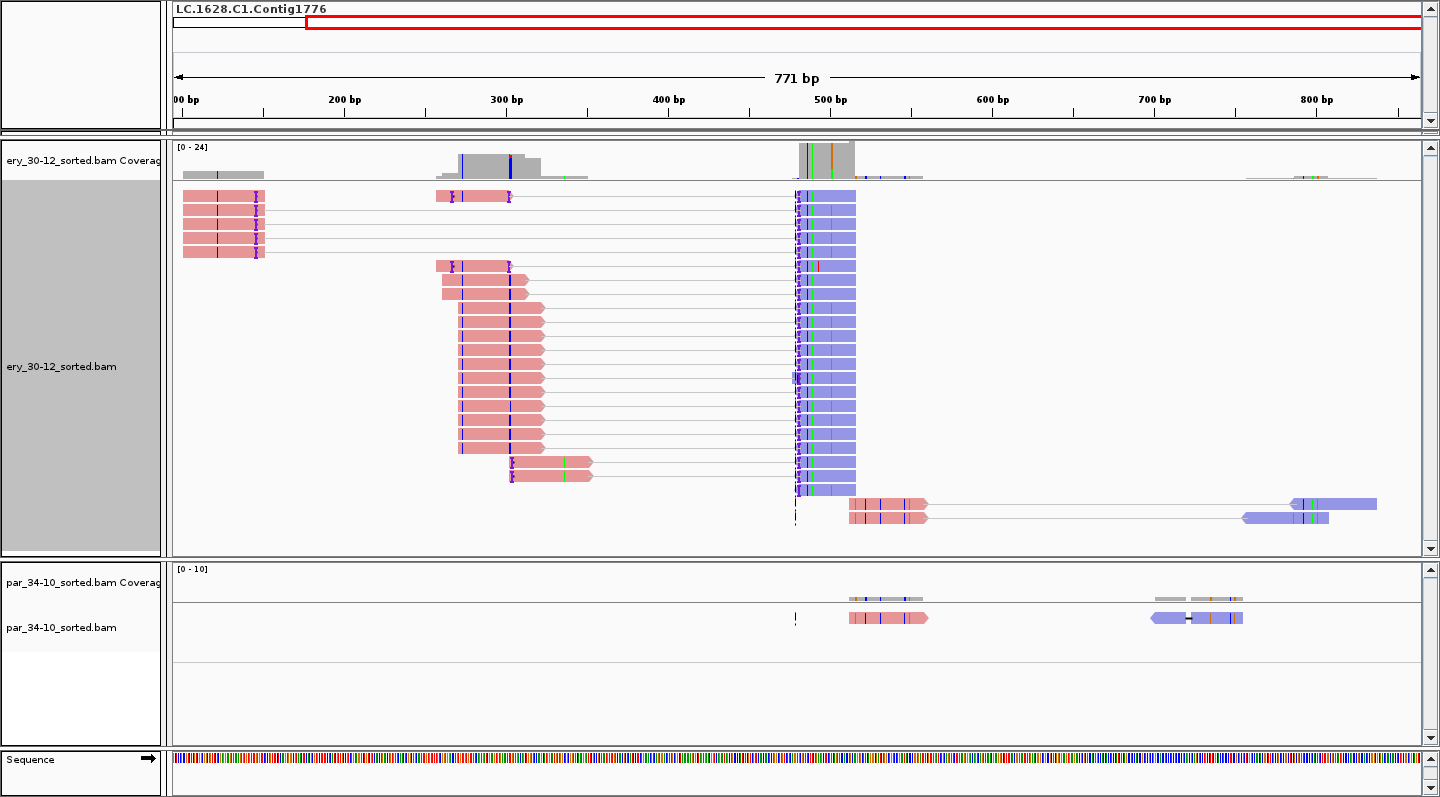
\includegraphics[width=\textwidth]{./figure/igv_LC_1628_C1_Contig1776_standRAD}
\caption{Alignment of standard RAD read pairs to both sides of an SbfI restriction site. Read pairs are connected by a line. The upper individual has 7 unique read pairs, i. e. with different paired-end reads.}
\label{LC.1628.C1.Contig1776_standRAD}
\end{figure}

\roger{Figure \ref{LC.1628.C1.Contig1776_standRAD} shows the alignment of standard RAD\footnote{SbfI restriction +  random shearing} reads against \textit{Schistocerca} contig LC.1628.C1.Contig1776 showing reads mapped to the same SbfI restriction site (centre) and their corresponding paired-end reads. The paired-end reads on both sides of the SbfI site can be used to design primers for qPCR. In the upper alignment window for individual ery\_30-12, PCR duplicates can be inferred from read pairs having the same alignment position for their paired-end reads.}

The lower individual in figure \ref{LC.1628.C1.Contig1776_standRAD} has only one read pair. Their first bit has not been set (value 2). They have SAM flags 97 and 145, respectively. So it is an "improper pair". However, the two reads have a combined mapping quality of 16, they are correctly oriented and 243 base pairs apart. According to the \texttt{stampy} log file, the mean insert size it estimates is 98.4 bp with 34.5 standard deviations. Five standard deviations above the mean is 270. So I don't understand why this read pair didn't get the "proper pair" bit flag set. 

I contacted Gerton Lunter, the author of \texttt{stampy}, about this. It turns out that \texttt{stampy} does not set the "proper pair" flag if the insert size is more than 3 standard deviations (not 5 as stated in the README file) away from the mean of the inferred insert size distribution. Since in these mapping trials, only a few reads map as a pair, it is probably best to turn off \texttt{stampy}'s inference of the insert size distribution and instead specify a very broad one. Then unusually large or small insert sizes will not prevent the setting of the "proper pair" flag. Suspicious insert sizes can easily be filtered out with \texttt{awk} or \texttt{perl} and read pairs with false orientation won't have the "proper pair" flag.

I have rerun the newest version of \texttt{stampy} on the standard RAD reads of the two individuals with the switch \texttt{--noautosense} to turn off inference of insert size distribution and \texttt{--insertsd=400} to specify a very wide insert size distribution. The output files are in \\{\scriptsize{ \texttt{/data/claudius/Read\_mapping/Schistocerca/mapping\_standard\_RAD\_reads/with\_stampy-1.0.23/large\_insertsd} }}.

I used command \ref{convert_sam_to_bam} with the modification "-F12" and "-q4" to create sorted bam files from the output of \texttt{stampy}. When I used "--processpart" with \texttt{stampy} I merged the sorted bam files with the "samtools merge" command into one bam file for each individual.

\roger{Visually inspecting all contigs with \texttt{IGV} for whether they have read pairs mapped to both sides of one SbfI restriction site is very tedious and time consuming. So I wrote a script called \texttt{find\_linked\_RADtags.pl} which reports reference contigs where at least two read pairs map to opposite sites of an SbfI restriction site (or any cut site leaving a 4 bp overhang). This script also detects the contig shown in figure \ref{LC.1628.C1.Contig1776_standRAD}. With this script the detection of a reference contig requires one "properly" mapped read pair on either side of an SbfI restriction site. So SE as well as PE reads need to map on both sides of the restriction site. This is stringent and will obviously miss contigs with genuine SbfI RADtag sites, but it is necessary to remove many false positive detections. The purpose of the script is not to detect as many contigs as possible, but only to detect several contigs with genuine SbfI RADtag sites.}

\begin{table}
\centering
\caption{List of \textit{Schistocerca} contigs that contain paired reads mapped to the same SbfI restriction site.}
\begin{tabular}{l}
\toprule
LC.148.C1.Contig208 \\
LC.637.C1.Contig745 \\
LC.637.C2.Contig746 \\
LC.1094.C1.Contig1233 \\
LC.1628.C1.Contig1776 \\
LC.2844.C1.Contig3004 \\
LC.3629.C1.Contig3766 \\
LC.4054.C1.Contig4181 \\
LC.4466.C1.Contig4569 \\
LC01024A1G12.f1 \\
LC03001A1D08.f1 \\
LC03001B1D09.f1 \\
\bottomrule
\end{tabular}
\label{linked_RADtag_contigs}
\end{table}

\roger{Table \ref{linked_RADtag_contigs} lists the contigs that could be found with the script and after inspecting the alignments in IGV.}

%%%%%%%%%%%%%%%%%%%%%
\subsection{\textit{Timema} as reference}
%%%%%%%%%%%%%%%%%%%%%

\begin{table}[h!]
\centering
\caption{List of \textit{Timema} contigs that contain paired reads mapped to the same SbfI restriction site.}
\begin{tabular}{l}
\toprule
lgNA\_ordNA\_scaf6294 \\
\bottomrule
\end{tabular}
\label{linked_RADtag_contigs_Timema}
\end{table}

%%%%%%%%%%%%%%%%%%%%%%%%%%%%%%%
\section{\textit{de novo} assembly of paired-end reads}
%%%%%%%%%%%%%%%%%%%%%%%%%%%%%%%
\roger{In order to design PCR primers I need to assemble the paired-end reads from single-end reads that map to the same restriction site. The \texttt{find\_linked\_RADtags.pl} script required at least one properly mapped read pair on either side of a restriction site to detect a contig. Instead of only taking paired-end reads from properly mapped pairs for the assembly, I also want to take unmapped paired-end reads that belong to single-end reads that mapped to the same restriction site.}

I could modify and extend the \texttt{find\_linked\_RADtags.pl} script to not only report reference contigs with linked RAD tags but also collect and safe all associated paired-end reads. I should do this in a \texttt{git} branch. I created a branch called \texttt{paired\_end} in my \texttt{scripts for RAD} repository on huluvu, in order to be able to safely modify the \texttt{find\_linked\_RADtags.pl} script without risking to destroy the previous working copy. \roger{The new script now collects all paired-end reads that are mates of single-end reads that mapped to a detected "linked RAD tag" site. It prints reads upstream or downstream of that site to separate files for each detected reference contig. These files can then be used as input to a \textit{de novo} assembler.}

%%%%%%%%%%%%%%%%%%%%%%%%%%%%%%%

\subsection{\texttt{Velvet}}
I used \texttt{VelvetOptimiser.pl} to assemble the collected paired-end reads into PE contigs. I wrote a wrapper script that runs \texttt{VelvetOptimiser.pl} on all input files in series\footnote{The low processor and memory usage of \texttt{velvet} on these input files indicates that it is read/write limited due to the many temporary files it creates.}. I adapted it from a script that John Davey gave me called \texttt{output\_rad\_paired\_end\_contigs\_velvetoptimiser.pl}. It writes contig files with more informative headers.

The assembler fails to assemble three PE contigs: Contig1776\_downstream, Contig4139\_upstream, LC03019A1F03.f1\_upstream. Contig 1776 is shown in fig. \ref{LC.1628.C1.Contig1776_standRAD}. I don't know why the assembly of the downstream PE contig fails on this \textit{Schistocerca} transcriptome contig other than due to insufficient coverage. I don't know how to tell \texttt{velvet} via \texttt{VelvetOptimiser.pl} that one read is enough evidence to extend a contig. Setting "-exp\_cov 1" and "-cov\_cutoff -1" doesn't improve the assembly.

I wrote a little script \texttt{select\_longest\_contig.pl} that picks the longest contig from each of the output files of \texttt{wrap\_velvetoptimiser.pl}. They could now be fed into \texttt{Primer3} for PCR primer design.
%\vspace{10pt} \\

%%%%%%%%%%%%%%%%%%%%%%%%%%%%%%%

\subsection{Eric Johnson's PE assembly}
\label{Eric Johnson's PE assembly}
\citet{Etter2011} did local de novo assembly of paired-end reads. They did paired-end sequencing of a standard SbfI RAD library of two stickleback individuals. Eric Johnson wrote custom Perl scripts which cluster SE reads by read sequence identity via hash assignment and then use \texttt{velvet} for each set of paired-end reads. He discards loci with less than 30 and more than 1000 reads. He then maps reads back to the PE contigs and calls SNP's again with a custom Perl script  (which is not published). They also created several partial digest libraries with \texttt{E. coli} and were able to assemble overlapping PE contigs covering the whole genome. They also created long-insert RAD paired-end libraries via two circularisation steps during the library prep. With this data they were able to assemble PE reads between 1 and 6 kb away from the cut site into contigs of several thousand base pairs length. They used a quite smart strategy for the assembly of the long-insert PE contigs:
\begin{quote}
\textsf{We took an additional computational step by first assembling the short reads with a long word length of 41, then assembling the short reads again with a shorter word length that depended on coverage and used the contigs produced by the first assembly as long reads to help bridge repeats in the sequence.}
\end{quote}
Adapting the word length (=hash length, =kmer length) to the coverage, i. e. number of reads per local de novo assembly, could be a trick to avoid trying out assemblies with a range of kmer lengths with \texttt{VelvetOptimiser.pl}, which is a very slow process.

\texttt{Velvet}'s kmer length is the length of sequence that needs to match (with x number of mismatches and deletions) between two reads in order to join them. I could recompile \texttt{Velvet} with a MAXKMERLENGTH of the same length as the read length for RADseq assembly. That way, \texttt{Velvet} would not be able to falsely extend RAD reads into longer bogus contigs but instead would only cluster.\footnote{I think this won't work, since a subsequence of kmer size length needs to match between two reads in order to join them. Setting the kmer size to the read length, only identical reads will be joined.}
\vspace{10pt}

%%%%%%%%%%%%%%%%%%%%%%%%%%%%%%%

\subsection{\texttt{SSAKE}}

\roger{\texttt{SSAKE} does not take base quality scores into account and takes only multi-fasta files as input. It searches for \emph{perfect} kmer matches between reads. i. e. does not allow for sequencing error or SNP's \citep{Warren2007}. }
I created a folder called "SSAKE" for experiments in: \\
{\scriptsize{
\texttt{/data/claudius/Read\_mapping/Schistocerca/mapping\_standard\_RAD\_reads/with\_stampy-1.0.23/large\_insertsd/ery\_30-12}
}}
In that folder, I used command \ref{fastq_to_fasta} to get fasta versions of the fastq files that were created by \texttt{find\_linked\_RADtags.pl}:

\begin{command}
\captionsetup{type=command}
\begin{Verbatim}[fontsize=\footnotesize]
for i in ../*fq; do awk '(NR-1)%4==0 || (NR-2)%4==0' $i | sed 's/^@/>/' > `basename $i .fq`.fa; done
\end{Verbatim}
\caption{Command line that takes all fastq files in the parent directory, extracts the header and sequence part (while skipping the quality string), replaces the "@" at the beginning of the fastq headers with a required ">" sign and writes the stream to a new file with the same base name.}
\label{fastq_to_fasta}
\end{command}

\roger{\texttt{SSAKE} by default does not allow a minimum overlap (-m) less than 16 bp. This could be too stringent for some of the low coverage PE contigs that I want to assemble. I modified \texttt{SSAKE} to allow a minimum overlap of as small as 10 bp. When calling \texttt{SSAKE} with \texttt{-w 1} and \texttt{-o 1} on the "Contig1776\_downstream" reads for PE assembly (just two overlapping reads, see fig. \ref{LC.1628.C1.Contig1776_standRAD}), it is able to assemble a full length contig of 81 bp length.} This is the behaviour that I wanted. \texttt{SSAKE} requires a perfect match of overlapping reads in order to merge them. Given low coverage and reads from a polymorphic sample, SNP's and indels could prevent a contig extension. See line 999 onwards in \texttt{SSAKE} to change this. One possibility would be a simple mismatch count, another one a full Needleman-Wunsch global alignment that could also handle indels.

(07/03/2014)\\
\roger{I have mapped the standard RAD reads of all 36 individuals against the \textit{Schistocerca} transcriptome with \texttt{stampy} in sensitive mode (see \texttt{Schistocerca.sh}) in order to achieve higher coverage for the assembly of PE contigs around detected linked RAD tag sites. The mapping of the paired reads of all 36 individuals from the  "Big Data" standard RAD library took 6h 24m.}

\begin{command}
\captionsetup{type=command}
\begin{Verbatim}[fontsize=\footnotesize]
for i in *sam.gz; \
do (samtools view -hS $i | gawk '/^\@/ || and($2, 4)==0 || and($2, 8)==0' | \
samtools view -uhS - | samtools sort - `basename $i .fq_1.sam.gz`) & done
\end{Verbatim}
\caption{Command line that uses \texttt{samtools} and \texttt{awk} to create position sorted bam files in parallel that only contain records of paired reads where at least one read of the pair got mapped (i. e. skipping records with flag 77 and 141). \scriptsize{Note the brackets around the command line and the skipping of ";" between "\&" and "done"}. }
\label{sam_to_bam_via_awk_in_parallel}
\end{command}

I used command \ref{sam_to_bam_via_awk_in_parallel} in order to extract all SAM records, where at least one read in a pair got mapped, with subsequent position sorting. I could not use GNU \texttt{parallel} in order to parallelize the sam to bam conversion including \texttt{awk} filtering. Sending each instance of the \texttt{for} loop into the background (thus parallising) greatly speeds up this task on huluvu (from 10 minutes to 30 seconds). 

\textbf{Running \texttt{stampy} in sensitive mode had virtually no effect on the number of reads that got mapped.}

I modified \texttt{find\_linked\_RADtags.pl} to only output PE reads whose SE mates mapped to a RADtag site.

\roger{The Big Data standard RAD reads used here (as in the previous section) were \texttt{process\_radtags} purified with a quality score threshold of 20 in a 20 bp sliding window. I merged all individual bam files into one big bam file with \texttt{samtools merge} and ran \texttt{find\_linked\_RADtags.pl} on it. That way, I get the PE reads from all individuals that belong to a linked RADtag site that was detected in as little as one individual (with a "properly mapped" pair on either side of the restriction site, see above).}

\roger{Running \texttt{find\_linked\_RADtags.pl} on the \texttt{all\_big\_Data.bam} (427Mb) took 25 minutes. It detected 77 reference contigs.} \texttt{SSAKE} requires a perfectly matching overlap and the author recommends quality trimming reads for that reason. So I have combined all reads that \texttt{find\_linked\_RADtags.pl} has output and have run \texttt{fastqc} on it. Note that the bam files created by \texttt{stampy} contain Sanger +33 quality strings. The quality score format of the original input fastq files was Solexa +64. Figure \ref{per_base_quality} shows that quality trimming of those reads for \texttt{SSAKE} should not be necessary.

\begin{figure}[htb]
\centering
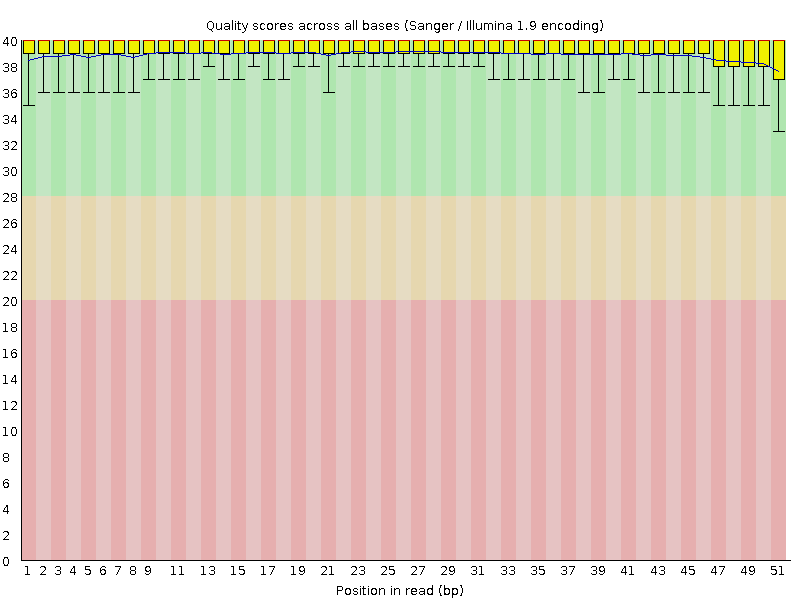
\includegraphics[width=.8\textwidth]{./figure/per_base_quality}
\caption{The quality score distribution of all reads that \texttt{find\_linked\_RADtags.pl} has output. It is very good. So quality trimming should not be necessary. Note that the quality score format has been changed to Phred +33 by \texttt{stampy}.}
\label{per_base_quality}
\end{figure}

Any non-genomic sequence should interfere with de novo assembly, so I need to get rid of it. Kang-Wook has written a nice Perl script called \texttt{TagCle} that detects overlap between paired read sequences by Smith-Waterman local alignment and clips off read segments downstream of the end of the local alignment, i. e. generally adapter sequence. So this script can also detect a single adapter (or barcode) base at the end of a read. 

The script \texttt{find\_linked\_RADtags.pl} outputs the SE as well as PE reads that belong to a detected linked RAD tag site into one file. I used command \ref{allocate_records} to write SE and PE records from that output file to separate files.

\begin{command}
\captionsetup{type=command} % this is necessary for the hyperlink to work, see manual for caption package, 6.5 about hyperref
\begin{Verbatim}[fontsize=\footnotesize]
$ grep -A3 "_2$" all_reads_for_PE_assembly.fq | grep -v "^--$" > all_reads_for_PE_assembly.fq_2
$ grep -A3 "_1$" all_reads_for_PE_assembly.fq | grep -v "^--$" > all_reads_for_PE_assembly.fq_1
$ for i in ../*fq; do grep -A3 "^@.*_2$" $i | grep -v "^--$" > `basename $i`_2; done &
\end{Verbatim}
\caption{Commands that allocate fastq records from a fastq file containing SE as well as PE records into separate files. SE records should have a header/ID line ending with "1" and PE records ending with "2".}
\label{allocate_records}
\end{command}

I put Kang-Wook's \texttt{TagCle} script into a new git branch called "tagcle" of my repository \texttt{scripts\_for\_RAD} in order to be able to track my changes to it. Note, that this script can only be called when the git branch "tagcle" is checked out. The other git branches do not contain this script.

I needed to change \texttt{find\_linked\_RADtags.pl}, so that it outputs reads that \texttt{stampy} had reverse complemented (in the SAM output) in their original orientation. Only then does Kang-Wook's script work correctly. I created a separate folder called \texttt{TagCle} and used command \ref{allocate_records} in order to put all input files in it.
I then ran \texttt{TagCle} as shown in command \ref{tagcle_run}. This took only ca. 5 to 10 minutes. 

\begin{command}[htb]
\captionsetup{type=command} % this is necessary for the hyperlink to work, see manual for caption package, 6.5 about hyperref
\begin{Verbatim}[fontsize=\footnotesize]
$ for i in ../input/*fq_1; 
do (j=`echo $i | sed 's/1$/2/'`; TagCle_0.70.pl -me -i1 $i -i2 $j > `basename $i .fq_1`.log ) & 
done
\end{Verbatim}
\caption{The command line that I used in order to run Kang-Wook's script \texttt{TagCle} on all 154 pairs of input files in parallel. The \texttt{-me} switch turns off any direct search for adapter sequences.}
\label{tagcle_run}
\end{command}

\texttt{TagCle} clipped 159 SE and 216 PE reads of a total of 1,584,732 reads (0.02\%). It did not discard any sequence. \texttt{TagCle} also quality trimmed with a Phred quality threshold of 20 in a 10bp window (\texttt{process\_radtags} had applied a 20bp window).

Since I want to use PE as well as SE reads for the de novo assembly, I had to combine the \texttt{TagCle} output files for SE and PE reads. I did this for all 154 paired \texttt{TagCle} output files with command \ref{combine_seqs}.

\begin{command}[htb]
\captionsetup{type=command} % this is necessary for the hyperlink to work, see manual for caption package, 6.5 about hyperref
\begin{Verbatim}[fontsize=\footnotesize]
$ for i in *fq_1; do j=`echo $i | sed 's/_1$//'`; cat $i "$j"_2 > $j; done &
\end{Verbatim}
\caption{Command that concatenates SE and PE files containing reads upstream or downstream of a RADtag site for each detected contig}
\label{combine_seqs}
\end{command}

\roger{The reads are now ready for de novo assembly. I ran command \ref{SSAKE} to do the de novo assembly for all upstream or downstream regions of a detected RAD tag site.}

\begin{command}[htb]
\captionsetup{type=command} % this is necessary for the hyperlink to work, see manual for caption package, 6.5 about hyperref
\begin{Verbatim}[fontsize=\footnotesize]
$ parallel 'SSAKE -f {} -w 1 -o 1 -m 15 -c 1 2&>1 > /dev/null' ::: *fa
\end{Verbatim}
\caption{Command to run the de novo assembler \texttt{SSAKE} in parallel on all fasta files. The minimum perfect overlap for an extension is 15 bp and 1 read is enough prove to make that extension. No contig clipping due to low coverage at the ends.}
\label{SSAKE}
\end{command}

\roger{\texttt{SSAKE} generally assembles many contigs for a region. In some cases this is due to different SE RADtags mapping to the same position in the \textit{Schistocerca} transcriptome. In other cases, this is clearly due to insufficient merging of contigs by \texttt{SSAKE} due to low coverage and SNPs (fig. \ref{contig_alignment}).} 

\begin{figure}[htb]
\centering
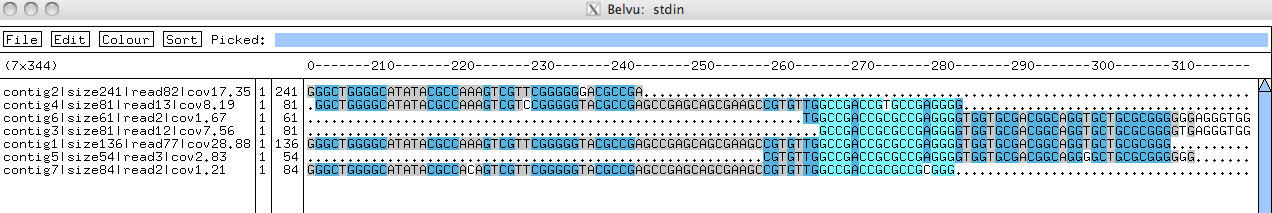
\includegraphics[width=\textwidth]{./figure/contig_alignment}
\caption{Multiple sequence alignment of \texttt{SSAKE} contigs assembled from reads collected from the downstream side of the RADtag site in the \textit{Schistocerca} reference contig "LC.1628.C1.Contig1776". The aligment was created with the command: \texttt{muscle -in *LC.1628.C1.Contig1776\_downstream*contigs -msf | belvu -}~. The 7 contigs can clearly be merged into one big contig if allowing for a few SNP's.}
\label{contig_alignment}
\end{figure}

\roger{\textbf{So, how can I pick those upstream and downstream PE-contigs that truly belong to the same RADtag site?} }I modified \texttt{find\_linked\_RADtags.pl} to insert "pp" into the fastq header of collected PE reads if they were mapped in a proper pair by \texttt{stampy}. \texttt{SSAKE} outputs a .readposition file reporting for each assembled contig the fastq headers and position in the \texttt{SSAKE }contig of reads that were used for its assembly. I wrote a little Perl script \texttt{pick\_contigs.pl} that screens those .readpostion files for the occurrence of the "pp" flag. For most detected linked RADtags sites there exist several \texttt{SSAKE} contigs which used "properly mapped" reads. For only 3 RADtag sites this leads to the selection of one \texttt{SSAKE} contig on either side. 

%%%%%%%%%%%%%%%%%%%%%%%%%%%%%%
\subsubsection{Optimising kmer length for \texttt{SSAKE}}
%%%%%%%%%%%%%%%%%%%%%%%%%%%%%%

\roger{All de novo assemblers require optimisation of kmer length, which is mainly what \texttt{VelvetOptimiser.pl} does with \texttt{Velvet}. So I wrote a script called \texttt{SSAKEoptimiser.pl} which iterates through kmer lengths of 11 to 33 and keeps the assembly which produces the longest contig.} This script is in the git branch "paired\_end". I  ran it with GNU \texttt{parallel} on all 154 fasta files containing the \texttt{TagCle} cleaned SE and PE reads that \texttt{find\_linked\_RADtags.pl} has output. The script takes 1h 38m to complete. \roger{One disadvantage of this script is that it is not parallelised, i. e. for each input sequence file the \texttt{SSAKE} assemblies for each kmer length are done in series. So the script spends a long time using just one core for the assemblies of one very large input file. To address this shortcoming, I wrote 4 versions of a parallelised \texttt{SSAKEoptimiser.pl} script using the Perl modules MCE, Parallel::ForkManager (PFM), threads (thr), and Thread::Queue. The PFM version of the script only takes 17 minutes to complete with essentially the same output as the unparallelised version of the script, i.e for each input file it finds the same longest contig.} See the folder "SSAKEoptimiser" in my git repository for the four versions of SSAKEoptimiser using different Perl modules. \roger{All versions run with essentially the same speed (fig \ref{runtimes}).} See \texttt{/home/claudius/bin/scripts\_for\_RAD/SSAKEoptimiser/Runtime} on huluvu. Note that this folder only exists when the git branch "paired\_end" is checked out.

\begin{figure}[htb!]
\centering
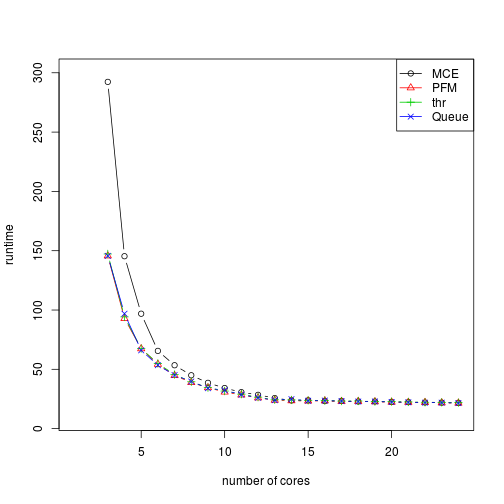
\includegraphics[width=.9\textwidth]{./figure/SSAKEoptimiser_runtimes}
\caption{The run times of the four parallelised versions of the \texttt{SSAKEoptimiser} script on 11 input files. An unknown bottleneck prevents further speedup beyond 15 cores. All scripts run with essentially the same speed except for very low core numbers.}
\label{runtimes}
\end{figure}

\roger{The optimisation of \texttt{SSAKE} assemblies by iterating through kmer lengths has markedly increased the length of the longest contig that could be assembled with reads that are associated with the downstream side of the RADtag site on the \texttt{Schistocerca} cDNA contig LC.1628.C1.Contig1776 (compare fig. \ref{contig_alignment} and fig. \ref{contig_alignment_opt}).}

\begin{figure}[htb!]
\centering
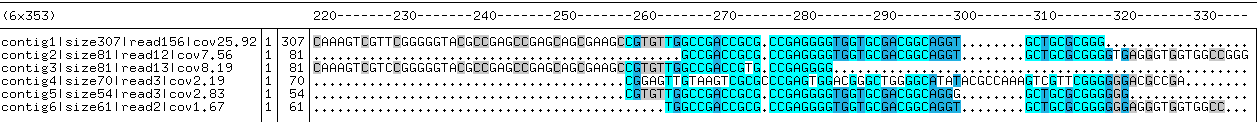
\includegraphics[width=\textwidth]{./figure/SSAKE_longest_contig}
\caption{Compare with figure \ref{contig_alignment}. \texttt{SSAKE} optimisation has increased the length of the longest contig with PE reads from the downstream side of the RADtag site on the \texttt{Schistocerca} contig LC.1628.C1.Contig1776.}
\label{contig_alignment_opt}
\end{figure}

\roger{I have taken the \texttt{SSAKE} contigs from the best assemblies of upstream and downstream paired-end reads associated with the RADtag site on \texttt{Schistocerca} reference contig LC.1628.C1.Contig1776 and have aligned them against the Schisto reference contig. Figure \ref{SSAKE_contigs_aligned_against_Schisto_contig} shows the alignment for the SSAKE contigs assembled on the downstream side. The reference sequence is reverse complemented. The longest \texttt{SSAKE} contig extends beyond the reference sequence. This is to check that the assembled upstream and downstream contigs actually belong to the same locus, i. e. RADtag site. I should do this check for all RADtag sites that I want to check for complete digestion with PCR. Also contig2 could clearly be merged with contig1, extending the longest contig by a few base pairs. I currently do not understand why \texttt{SSAKE} cannot make this extension. }

\begin{figure}[htb!]
\centering
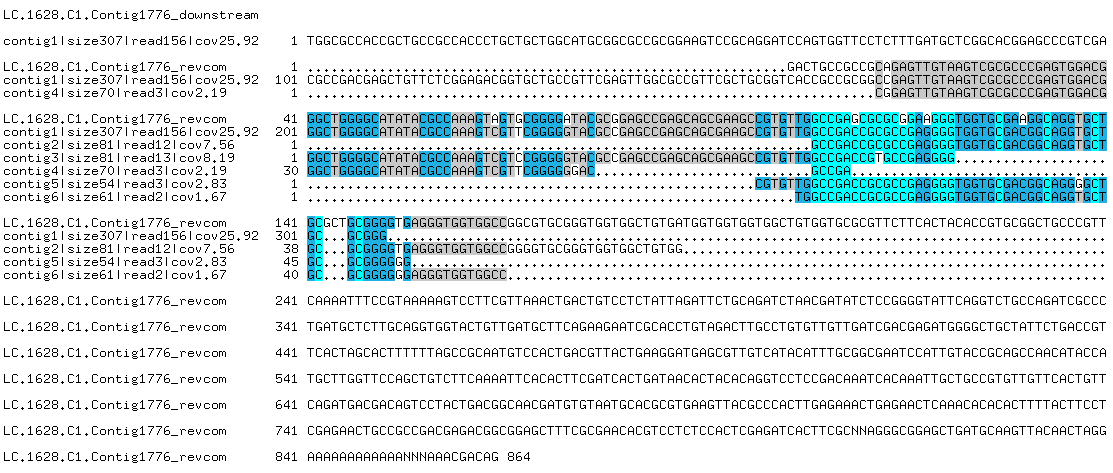
\includegraphics[width=\textwidth]{./figure/SSAKE_contigs_aligned_against_Schisto_contig}
\caption{Multiple sequence alignment of \texttt{SSAKE} contigs from the downstream side of the RADtag site on reference contig LC.1628.C1.Contig1776, including the reference contig.}
\label{SSAKE_contigs_aligned_against_Schisto_contig}
\end{figure}

\roger{Since the \texttt{SSAKEoptimiser} output generally contains several contigs of similar length and with similar read counts, it is difficult to pick those contigs upstream and downstream that genuinely belong together, i. e. come from the same locus. It is by no means always the longest contig assembled that aligns significantly to the Schisto reference (visual inspection of a muscle pairwise alignment).} That is why I tried to improve on the quality of the assembly. As described in \citet{Etter2011} for the \texttt{Velvet} assembler, I first did a \texttt{SSAKE} run with kmer size 41 on all input files. I then took the contigs of this \texttt{SSAKE} run and added them to the input files in order to run these new input files with \texttt{SSAKEoptimiser}. The idea is that an assembly with kmer size 41 only assembles genuinely contiguous sequences. Those conservative contigs could then inform a more permissive SSAKE run with smaller kmer size about when an extension is not consistent with one of the conservative contigs (see section \ref{Eric Johnson's PE assembly}). But how can I gauge the quality of the assembly. The sum of the lengths of the longest contigs for each input file is only marginally higher than for the normal \texttt{SSAKEoptimiser} output: 29712 to 29579. Also, using an only slightly modified version of \texttt{assemblathon\_stats.pl} on the concatenation of all *.contigs files shows that the two-step assembly produced only 53 contigs larger than 300 bp as compared to 65 with the one-step method. The number of contigs both methods assemble is not different and so is N50. I conclude that for these paired-end read assemblies, the two-step method of assembly does not provide a significant gain.

%%%%%%%%%%%%%%%%%%%%%%%%%%%%%
\subsubsection{Picking the right \texttt{SSAKE} contig}
%%%%%%%%%%%%%%%%%%%%%%%%%%%%%
\label{pick}

\roger{I did \texttt{muscle} alignments with all *contigs output files from the one-step \texttt{SSAKE} assemblies in order to manually merge \texttt{SSAKE} contigs in \texttt{MEGA}.\footnote{One *contigs file, for the upstream side of Schisto reference contig LC03010B1A12.f1, contains 11,560 \texttt{SSAKE} contigs and \texttt{muscle} was not able to complete the alignment for this file overnight. It would have been of no use anyway.} } I copied these alignment files to my Mac in order to open them in \texttt{MEGA} (see \verb!.../THESIS/data_analysis/reference-mapping/data!).
I also created a table in the file \verb!with_up-downstream_contig.SSAKE_contig_stats! that only contains information for Schisto contigs for which \texttt{SSAKE} was able to assemble an upstream and downstream contig. \roger{There are 64 Schisto reference contigs with a RADtag site for which at least one upstream and one downstream contig could be assembled.} The table lists for each *upstream|downstream*contigs file the length of the longest contig, the number of assembled contigs, the number of contigs >=100, >=200 and >=300.

\roger{An important piece of information for picking the right contig would be a \texttt{blast} hit of a \texttt{SSAKE} contig against its putative Schisto reference contig. So I extracted all 64 Schisto reference contig sequences (unigenes) from the \texttt{Schistocerca} reference file \textsf{LC\_unique.seq} with \texttt{samtools faidx} (see command \ref{reduced_reference}). Using the \textsf{.SSAKE\_contig\_stats} file as input to a new script called \texttt{blast2seq.pl}, I blasted all 128 relevant *contigs files against their putative Schisto reference contig sequence and recorded the number of blast hits as well as the headers of the 10 best \texttt{SSAKE} hitting contigs together with their e-value in the \textsf{.SSAKE\_contig\_stats} file. I imported this new table into a LibreOffice spreadsheet for better browsing and annotation. I used this table as a guide for picking and possibly merging SSAKE contigs in \texttt{MEGA}.} In the libreoffice file (.ods) I marked those Schisto contigs green for which I could successfully pick \texttt{SSAKE} contigs on both sides of the RADtag site. I exported consensus sequences from merged \texttt{SSAKE} contigs into fasta.

\begin{command}
\captionsetup{type=command}
\begin{Verbatim}
blastn -query *LC03012A1D06.f1_downstream.fa.ssake*.contigs \
-subject *LC03012A1D06.f1_downstream.fa.ssake*.contigs -task blastn \
-evalue 1e-10 -outfmt 6 | awk '$1 != $2' | sort -k3 -nk11 | awk 'NR%2' | less -S
\end{Verbatim}
\caption{This command line example is a very quick way to find out which sequences in a multi fasta file are similar to each other. It prints out hits of an all by all blastn of the sequences in a file. Note that query and subject get the same file. The first awk command removes hits against itself, the sort part brings reciprocal hits together and the second awk command keeps only one line for each pair of matching sequences.}
\label{blastn}
\end{command}

\roger{As an example of the \texttt{SSAKE} contig picking process, the assembly of paired-end contigs on the upstream side of Schisto reference contig LC.637.C2.Contig746 with \texttt{SSAKE} resulted in 50 contigs, 10 of size > 100, 2 of size > 200 and 1 of size > 300. Seven of the 50 contigs get a blast hit to the reference with evalue <1e-10. However, the longest \texttt{SSAKE} contig does not get a blast hit with the Schisto reference contig nor does it share similar subsequences with any of the 7 contigs that do get blast hits with the reference (determined from the output of an all vs all blastn as in command \ref{blastn}). \textbf{I only took the \texttt{SSAKE} contigs with blast hits against the reference for the generation of the consensus sequence.} }

I replaced the fasta header lines in the \texttt{SSAKE} contig consensus files with the names of these files using command \ref{fname_to_header}.

\begin{command}
\captionsetup{type=command}
\begin{Verbatim}
for i in *fas; do perl -i"bak" -ne'$ARGV=~s/\.fas$//; s/^>.*/>$ARGV/; print;' $i; done
\end{Verbatim}
\caption{This command replaces the fasta header line in the fasta file with the name of that file.}
\label{fname_to_header}
\end{command}

\roger{I then aligned upstream contigs and reverse complemented downstream contigs against their \texttt{Schistocerca} reference if possible (i. e. significant blast hit). I created a "primer3\_ready" sequence from upstream contig sequence and reverse complemented downstream contig sequence filling the gap between them with N's. I could create 20 "primer3\_ready" sequences, i. e. \textbf{for 20 \texttt{Schistocerca} cDNA contigs I could assemble and confidently pick down and upstream contigs for PCR primer design.} } 

%%%%%%%%%%%%%%%%%%%%%%%%%%%%%%%
\subsection{RepBase}
%%%%%%%%%%%%%%%%%%%%%%%%%%%%%%%

\roger{I am screening the consensus paired-end contig sequences against \href{http://www.girinst.org/server/RepBase/index.php}{RepBase}. } I downloaded the programme \href{http://www.girinst.org/downloads/software/censor/}{CENSOR} as well as the most recent version of legacy \texttt{blast} (i. e. not the new \texttt{blast+}). I also downloaded the newest version of RepBase and ran \texttt{CENSOR} with command \ref{censor_command}.

\begin{command}
\captionsetup{type=command}
\begin{Verbatim}
censor.ncbi ../all_20_primer3_ready_withoutBraces_sequences.fa -lib ang -lib dro -lib inv
\end{Verbatim}
\caption{This command runs \texttt{censor} against all 20 primer3\_ready sequences using repeat libraries of \textit{Anopheles gambiae}, \textit{Drosophila} as well as all "Invertebrates" (including protozoans and bacteria).}
\label{censor_command}
\end{command}

\roger{Using the 20 primer3\_ready sequences as input, \texttt{censor} finds 8 matches in 7 of them. \texttt{censor} also creates a .masked file, which contains the input sequences but with the detected subsequences masked out with a series X's.}

I have also submitted the 20 primer3\_ready sequences to the web service of \href{http://www.girinst.org/censor/index.php}{CENSOR} and selected "Hexapoda" as "sequence source". This resulted in only 3 sequences with a match to a repeat sequence in the database subset, one of which could not be found with the local censor run. The match to LC03012A1D06.f1\_primer3\_ready is also longer and to a different transposon than with the local \texttt{censor} run. The web service runs only with \texttt{wu-blast}, which is not freely available. I have downloaded the html output of the web service \texttt{censor} run. I think it is best to incorporate the additional masking from the web service run into the masking done by the local \texttt{censor} run.

%%%%%%%%%%%%%%%%%%%%%%%%%%%%%%%
\subsection{BatchPrimer3}
%%%%%%%%%%%%%%%%%%%%%%%%%%%%%%%

\roger{I am using the web based primer design programme \href{http://probes.pw.usda.gov/batchprimer3/}{\texttt{BatchPrimer3}} \citep{You2008}.}
\begin{epigraphs}
\qitem{
\textsf{
The best primers are selected based on the quality scores of candidate primers. The quality score is a weighted linear function of primer length, Tm, GC content, number of a single-base repeat and simple sequence repeats, number of an ambiguity code (N), and self-complementarity of the entire primer and the last 10 nucleotides in the 3' end. The maximum quality score of a candidate primer is 100. If the parameter values of a candidate primer are beyond the user-specified ranges, or a candidate primer contains single sequence repeats, the quality score is set to 0. Within specified parameter range, the closer the user-specified optimum value is to a calculated primer property value, the higher is the primer quality score. If the highest score is zero, no primer is given for the specified criteria.}
}
{\cite{You2008}, section "Web application design"}
\qitem{
\textsf{Generally, the score measuring the entire primer complementarity should be less than or equal to 8 and the score for 3' end complementarity should be less than or equal to 3.}
}
{\cite{You2008}, section "Parameter setting"}
\end{epigraphs}

\texttt{BatchPrimer3} has a neat feature to specify included, excluded and target regions for primer design:

\begin{epigraphs}
\qitem{
\textsf{
the "[]" pair can be used to specify targets, the "\{\}" pair to specify included region, and the "<>" pair to specify excluded region.
}
}
{from the \href{http://probes.pw.usda.gov/batchprimer3/}{website}}
\end{epigraphs}

I used command \ref{insert_square_brackets} in order to in order to mark the PCR target sequence with square brackets. Some primer3\_ready sequences also contain smaller stretches of N's that I introduced in order to connect two SSAKE contigs that mapped to their \textit{Schistocerca} cDNA reference. Command \ref{insert_square_brackets} deliberately skips them.

\begin{command}
\captionsetup{type=command}
\begin{Verbatim}[fontsize=\footnotesize]
perl -ne'if(/^>/){print}else{ s/([^N])(N{200,})/$1\[$2/g; s/(N{200,})([^N])/$1\]$2/g; print; }' \
all_20_primer3_ready_withoutBraces_combined_mask.fa
\end{Verbatim}
\caption{Perl command line that introduces square brackets around the long stretch of N's between the two PE-contig sequences. They are the target sequence, i. e. I want one primer on each side of the target.}
\label{insert_square_brackets}
\end{command}

I used a similar command to surround the stretches of "X" introduced by \texttt{censor} to indicate masked sequence with "<>", so that they are ignored by \texttt{BatchPrimer3} for primer design. \texttt{BatchPrimer3} also ignores stretches of N for primer design, so I did not explicitly mark them.

I have downloaded the \texttt{BatchPrimer3} script package from the website. It contains a \texttt{primer3\_core} version 1.1.1. This is quite an old version. In \texttt{BatchPrimer3} the T$_{m}$ is calculated using \texttt{primer3\_core}, which uses the \textit{nearest neighbor} method according to SantaLucia \citep{You2008}.

In figure \ref{BatchPrimer3_settings}, note the lower right input box in the upper "General settings" tab. It is the concentration of \textit{annealing} primer in nM, which is dependent on the template concentration, not the amount of primer that is added to the PCR mix. \roger{If I added 100 ng of grasshopper DNA to the PCR mix, assuming that the genome is 12 Gbp long, this would only correspond to 7604 template molecules for the primer. }

\begin{align}
\text{molar amount of template} = \frac{\text{amount of DNA}}{\text{MW of bp} \times \text{genome size}} \nonumber
= \frac{100 \times 10^{-9}g}{660 \frac{g}{mol \times bp} \times 12 \times 10^{9} \text{bp}} \nonumber
= 1.26 \times 10^{-20} \text{mol} 
\end{align}
\begin{align}
\text{number of template molecules} &= 1.26 \times 10^{-20} \text{mol} \times \text{Avogadro's number} \nonumber \\
&= 1.26 \times 10^{-20} \text{mol} \times 6.0221413 \times 10^{23} \nonumber \\
&= 7604 \nonumber
\end{align}

Certainly, at the beginning of the PCR, the concentration of annealing primers is much less than 50 nM, meaning that the actual T$_{m}$ will be much much lower than returned by \texttt{primer3}. 

Also note the non-default settings in the "Penalty Weights" tab at the bottom of figure \ref{BatchPrimer3_settings}. I put high penalties on complementarity of primers as well as primer pair melting temperature difference.

\begin{figure}[htb!]
\centering
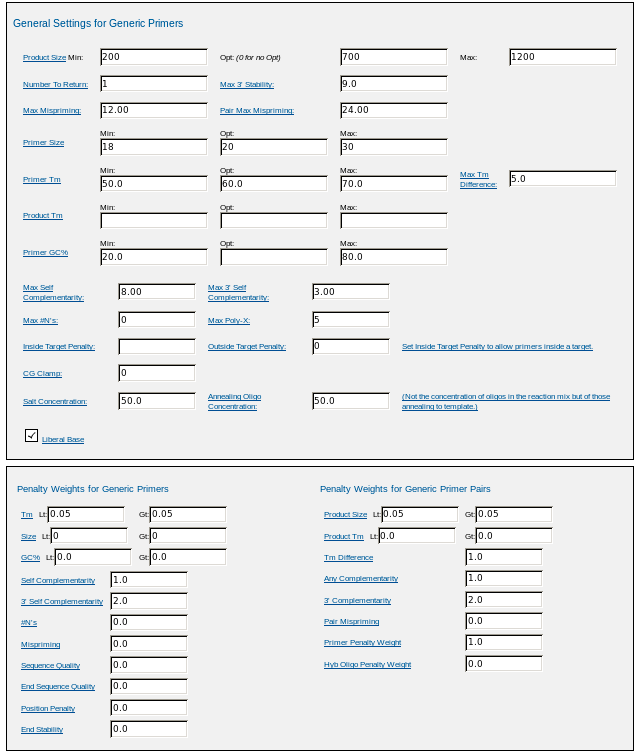
\includegraphics[width=\textwidth]{./figure/BatchPrimer3_settings}
\caption{Settings for the third \texttt{BatchPrimer3} run. }
\label{BatchPrimer3_settings}
\end{figure}

\roger{ \texttt{BatchPrimer3} was able to find suitable PCR primer pairs for all but one of the input sequences. The failure for one sequence was due to extensive repeat masking in the affected sequence (LC03012A1D06). }

I am going to use \href{https://www.neb.com/protocols/2012/09/06/protocol-phusion-high-fidelity-pcr-master-mix-with-hf-buffer-m0531}{Phusion Mastermix kit} as this comes with high quality dNTPs and better performance in general than Taq polymerase. According to the NEB documentation:

\begin{epigraphs}
\qitem{
\textsf{The NEB \href{https://www.neb.com/tools-and-resources/interactive-tools/tm-calculator}{T$_{m}$ calculator} should be used to determine the annealing temperature when using Phusion.}
}
{ \href{https://www.neb.com/protocols/2012/09/06/protocol-phusion-high-fidelity-pcr-master-mix-with-hf-buffer-m0531}{NEB Phusion Protocol} }
\end{epigraphs}

%%%%%%%%%%%%%%%%%%%%%%%%%%
\subsection{Mapping standard RAD reads back to PE contig sequences}
%%%%%%%%%%%%%%%%%%%%%%%%%%

\begin{comment}

\begin{itemize}
\item get single-end sequences that mapped to detected linked RADtags sites $\rightarrow$ TagCle input
\item create consensus sequences with \texttt{consambig} from \texttt{emboss} package
\item insert consensus of single-end RADtag sequences at correct position using alignment with \texttt{Schistocerca} reference contig $\rightarrow$ in MEGA
\item For the 40 tags for which I could assemble PE contigs on both sides of the restriction site, insert the single-end RAD tag sequence into the primer3\_ready sequence and map the Big Data RAD sequences of each individual against them. Single-end reads can be found as input to TagCle. Are there individuals for which only the tag on one side of the restriction site has been detected?
\end{itemize}

\end{comment}

\roger{I want to insert the single-end RAD tag sequences into the primer3\_ready sequences in order to use them as reference for a mapping of all reads of each individual. I want to examine how many individuals get reads mapped to those RADtag sites and whether individuals have reads mapped to both RAD tags at an SbfI restriction site or not. }

For the determination of the consensus single-end sequences I obviously only want to use reads whose mate was used for the assembly of the \texttt{SSAKE} PE-contig that I finally picked (see section \ref{pick}). That's because \texttt{find\_linked\_Radtags.pl} had printed out all paired reads that mapped to a detected linked RADtags site in the \texttt{Schistocerca} reference, but after the \texttt{SSAKE} assembly I mostly only picked PE-contigs that got a \texttt{blast} hit to their \texttt{Schistocerca} reference contig. Other \texttt{SSAKE} contigs are much more likely to derive from similar but non-homologous loci to the \texttt{Schistcerca} reference contig.

In the \texttt{Primer3} directory I created a subdirectory called \texttt{SE-sequences} where I put symlinks to the 40 single-end sequence files that \texttt{find\_linked\_RADtags.pl} had put out for the \texttt{Schistocerca} reference contigs for which I ultimately was able to create primer3\_ready sequences. In this subdirectory I created another subdirectory called \texttt{PE\_contigs} into which I put symlinks to the 40 PE contig consensus sequences that I used to create the 20 primer3\_ready sequences. I also put symlinks to the 40 corresponding PE read files into that directory. I then used command \ref{blast_mapping} in order to extract the fastq headers from those paired-end reads that get a blast hit to their inferred PE contig.

\begin{command}
\captionsetup{type=command}
\begin{Verbatim}
for i in *fq_2; \
do awk '(NR-2)%4==0 || (NR-1)%4==0' $i | sed 's/@/>/' | sed 's/_pp//' | \
blastn -subject `basename $i .fq_2`_consensus.fas -evalue 1e-10 -outfmt 6 | \
cut -f1 | sed 's/2$/1/' > `basename $i .fq_2`_blast_mapped.ids; \
done
\end{Verbatim}
\caption{Using \texttt{blastn} to find PE reads that map to the inferred PE contig (see section \ref{pick}). The \texttt{for} loop iterates over all 40 PE read files. The first part of the loop converts fastq to fasta format. The second line feeds that into \texttt{blastn} (using megablast by default) and uses the corresponding PE contig (from section \ref{pick}) as subject. The third line takes the first column with the query headers from the blast output table and writes it to an output file.
}
\label{blast_mapping} 
\end{command}

I can then use these *.ids files, containing headers of the required single-end sequences, as pattern files for a \texttt{grep} filter of the SE read files that \texttt{find\_linked\_RADtags.pl} has put out (see command \ref{grep_filter}).

\begin{command}
\captionsetup{type=command}
\begin{Verbatim}
for i in *ids; \
do grep -A1 -f $i ../all_Big_Data_`basename $i _blast_mapped.ids`.fq_1 | \
egrep -v "\-\-" | sed 's/@/>/' > `basename $i .ids`_SE.fas; \
done
\end{Verbatim}
\caption{Using the header files created by the previous command to extract corresponding SE reads from \texttt{find\_linked\_RADtags.pl} SE read files.}
\label{grep_filter}
\end{command}

I then created multiple sequences alignments with \texttt{muscle} in .msf format, which I could then use for the \texttt{consambig} programme from the \href{http://emboss.sourceforge.net/apps/release/6.6/emboss/apps/consambig.html}{\texttt{emboss}} package in order to create SE RADtag consensus sequences.

\texttt{find\_linked\_RADtags.pl} had also reported at which position in the \textit{Schistocerca} contig it had found a linked RADtag site. I am using this information together with the MEGA alignments of PE consensus sequences with their \textit{Schistocerca} contig to insert the SE RADtag sequences at the approximately right position. 

While inserting SE RADtag sequences into the primer3\_ready sequences, I found that the SE RADtags that map to \textit{Schistocerca} {\color{red}\textit{contig LC91.C2.Contig.134}} also map \emph{within} the downstream PE contig that I assembled for this "locus". That is dodgy and I should remove this locus from the primer3\_ready collection.

\roger{I have mapped all standard RAD reads of all 36 individuals against the "Primer3ready\_with\_RADtags" reference (created as described above) with \texttt{stampy}.} I specified a substitution rate of 0.01 (note that this is not a maximum error rate allowed, but rather an average error rate expected) and I filtered out unmapped reads and reads with a mapping quality score below 4 (which according to the \texttt{stampy} readme file are reads with ambiguous mapping locations).

\begin{figure}
\centering
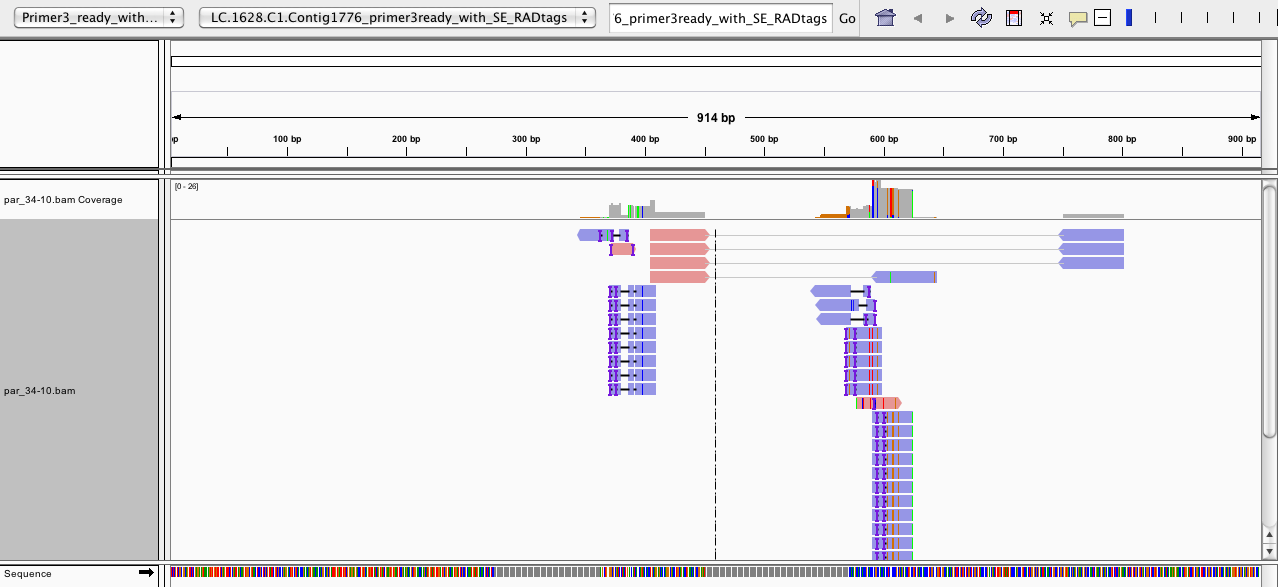
\includegraphics[width=\textwidth]{./figure/stampy_par_34-10_vs_primer3ready_igv}
\caption{Example read alignment of all standard RAD reads of individual par\_34-10 against one detected linked RADtags sequence in the primer3ready\_with\_RADtags reference.}
\label{stampy_par_34-10_vs_primer3ready_igv}
\end{figure}

\roger{Figure \ref{stampy_par_34-10_vs_primer3ready_igv} shows an example of alignment of this \texttt{stampy} mapping. There are many low quality mappings which are very likely wrong (e. g. SE reads mapped to PE contig without SbfI site). However, here I have been using reads derived from a much larger source than is represented in the small reference of 20 linked RADtags sites. Therefore, \texttt{stampy} finds unambiguous mapping locations (indicated by a mapping quality >3) for reads that have an edit distance of 17 to the reference sequence. \texttt{stampy} does not have an option for maximum allowed distance to the reference.}

The \texttt{stampy} README file does not mention how it handles ambiguity codes in the reference sequence (i. e. IUPAC symbols). Are they converted to N for mapping, are they scored as mismatches or as matches? Unfortunately \texttt{stampy} does not produce an MD tag \citep[p. 6]{SAMformatSpec2011}, which would indicate where in the read sequence mismatches and indels were detected. I have run a small subset of 250k reads from individual par\_34-10 from the standard RAD library once against the primer3 ready sequences including all ambiguity codes and once against this reference with the ambiguity codes RWYMKS replaced by N. Figure \ref{stampy_align_test} shows the alignment of the same read in the two \texttt{stampy} test runs. There does not seem to be a mismatch. Still \texttt{stampy} reports 2 or 3 mismatches, even though there are 4 ambiguity codes in the reference covered by this read.

\begin{figure}
\centering
\begin{subfigure}[b]{.9\textwidth}
\caption{with IUPAC symbols in reference}
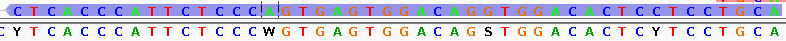
\includegraphics[width=\textwidth]{./figure/stampy_align_test_IUPAC_ref}
\label{IUPAC_ref}
\end{subfigure}
~
\begin{subfigure}[b]{.9\textwidth}
\caption{with IUPAC symbols converted to N in reference}
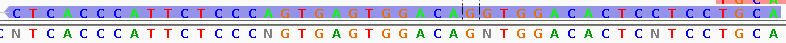
\includegraphics[width=\textwidth]{./figure/stampy_align_test_IUPAC_to_N_ref}
\label{IUPAC_to_N_ref}
\end{subfigure}
\caption{Comparing \texttt{stampy} alignments with different reference sequences. The same read is shown in (a) and (b). In (a) the edit distance to the reference that \texttt{stampy} reports is 2, in (b) it is 3 (from NM tag, see \citealt{SAMformatSpec2011}).}
\label{stampy_align_test}
\end{figure}

\roger{I therefore decided to test alternative mapping programmes. I am trying to produce so-called ROC curves with simulated read data for a couple of promising mapping programmes as done by \href{http://lh3lh3.users.sourceforge.net/alnROC.shtml}{Heng Li}. } I have downloaded the \textit{Heliconius melpomene} genome sequence into: \\

{\footnotesize{\texttt{/data/claudius/PE\_contigs/Primer3/mapping\_against\_primer3ready\_seqs/alignment\_tests/simulation}}} \\

I also cloned the git repo for \href{https://github.com/lh3/wgsim}{\texttt{wgsim}} into this directory. 

%%%%%%%%%%%%%%%%%%%%%%%%%%%%%%%%%%%%%%
\subsubsection{Mapping tool test}
%%%%%%%%%%%%%%%%%%%%%%%%%%%%%%%%%%%%%%

I did read \cite{Hatem2013}. Despite their use of different read simulators and reference genomes, different read lengths, different mapping programmes and a real dataset, it falls short of providing a convincing measurement of alignment accuracy. Like \cite{Holtgrewe2011}, they claim that, when using simulated read data, using the known origin of the read would be inadequate. But this is only inadequate if false positive mapping rate would be taken as an absolute measure. It is perfectly valid when comparing different programmes on the same simulated input read dataset. The reason why the authors of \cite{Hatem2013} think that using the known read origin for false positive estimation is inadequate is that in rare cases SNP's and sequencing errors can make a read more similar to another than its source location. They claim that if a read mapper reports that more similar location it has not produced a mapping error. In the real world, however, this would still be an error, even though not the fault of the mapping programme (but of evolution and the DNA sequencing process). What I want to get in such a case is an informative mapping quality score telling me there are several suboptimal alignment positions so that certainty in the reported location is reduced. \cite{Hatem2013} also falls short of providing a suitable mapping accuracy test with a real data set. \emph{Capture-sequence reads} or \emph{reads from pooled PCR products}, i. e. data with known origin, could have been used. As an alternative, \emph{paired-end read data could have been mapped in single-end mode and discordantly mapped read pairs counted.} A couple more shortcomings are mentioned in \href{http://lh3lh3.users.sourceforge.net/false-bench.shtml}{Flawed Benchmark on Aligners}.

The \href{http://www.seqan.de/projects/rabema/manual/#toc-using-rabema-in-normal-mode}{rabema} benchmark method \citep{Holtgrewe2011} in "oracle" mode, i. e. with simulated read data and known read origin is equivalent to using the \texttt{wgsim\_eval.pl} script of Heng Li and allowing $\pm$\textsf{read length} bps for the reported mapping location. Creating a "gold standard" from real data with \texttt{Razers3} is prohibitive in terms of time when using >100,000 reads and an allowed edit distance of >10\%. However, \roger{with reads longer than 50 bps, indels can easily cause an edit distance of >10\%. Only mapping tools that have a local alignment step and determine valid mapping locations based on alignment score instead of edit distance should still be able to correctly map such reads.} So the \texttt{rabema} benchmark method is unsuitable for modern read lengths and higher polymorphism rates, i. e. higher divergence of reads from the reference sequence than encountered when resequencing human genomes.

\cite{Ruffalo2011}, unfortunately, compare quite old versions of mapping programmes. They provide plots of \textsf{accuracy} over different degrees of polymorphism, i. e. error/SNP rate, indel rate and indel size. Their own definition of \textsf{accuracy} is the proportion of correctly mapped reads among all mapped reads, which is just 1 - \textsf{false positive rate}. So, here, it is identical to \textsf{precision}. The problem is that accuracy alone does not describe a detector completely. It needs to be put in relation to its \textsf{sensitivity}, i. e. \textsf{true positive rate}. Their plots of "used reads ratio" over error rate is no measure of sensitivity at all. That is if a read mapper provides a mapping location for all input reads, but all locations are wrong, even though it's "used reads ratio" is 1 it's sensitivity is zero, i. e. it was not able to detect any correct location. Note that \cite{Li2013} makes the same mistake. 

The \textit{ArtificialFastqGenerator} can only simulate sequencing errors \citep{Frampton2012}. It cannot simulate a divergent genome and then sample reads from this. Instead it randomly introduces sequencing errors, which can be based on base call quality scores of real reads. I could not find an explanation of how indels are simulated. So, \textit{ArtificialFastqGenerator} is designed to test a pipeline for false positive variant calls, not for false negative variant calls. For my low coverage mapping tool tests, sequencing errors should mirror polymorphisms, but I do not see any reason for trying out this simulator.

\roger{\cite{Palmieri2009} showed already that expression profiling is greatly affected by the mapping software, especially when dealing with a divergent reference sequence and a complex genome. Estimating allele frequencies from pooled DNA should be analogous to gene expression analysis and when coming from genomic DNA instead of RNA with the added complication of a more complex reference sequence.}

\cite{Lee2012a} have come up with a measure of how confident reads can be mapped that come from a particular region of the genome using \texttt{BWA}'s mapping quality scores, which should be a Phred scaled estimate of the probability that the read was mapped to a wrong location. \roger{Interestingly, for the human genome and even with 2000 bp long simulated PacBio reads with only 0.33\% error rate, more than 8\% of the genome have a "genome mappability score" (GMS) of less than 50\%, which corresponds to a mapping quality score of 3 or less. The GMS for a nucleotide position in the genome is the average "mapping probability" of any possible spanning read for that position and the mapping probability is the probability that a read was mapped to the correct location.} This is a slightly more sophisticated method to measure mappability than what was used for the \href{http://genomebrowser.wustl.edu/cgi-bin/hgTrackUi?db=hg18\&g=wgEncodeMapability}{\textit{broad mappability track}}.

\roger{\cite{Kosugi2013} have developed a few Perl scripts that deal with the problem of false positive alignments especially when doing a so-called "targeted alignment"\footnote{when the reference sequence is much smaller than the source of the reads to be mapped} by removing reads that map with too high a number of mismatches. They show that filtering by mapping quality score is rather ineffective when trying to improve a targeted alignment. Their figure 3 shows before and after IGV read alignment views of whole genome reads aligned against one chromosome or even just 1 Mbp region. This is the problem that I face with mapping all RAD reads against 20 "linked Radtags + PE contigs" reference sequences. I could use their \texttt{Coval-Refine} script to filter out read mappings with too many mismatches.}  
They have also developed their own variant caller, which seems to perform as well as \texttt{samtools} or \texttt{GATK}. They also demonstrate a neat way to use simulation and empirical data together in order to determine false positive and false negative rates. They simulate a mutated reference sequence and then map empirical reads against it. Before that they try to remove as many real (i. e. not simulated) SNP's/indels from the empirical reads as possible, which would otherwise be counted as false positives. Even though this method tends to give over-estimated false positive rates, this is certainly good enough when comparing different programmes. They show that reads simulated from a reference sequence are generally mapped much more accurately, i. e. with much lower number of mismatches, than empirical reads. I agree with that, even if divergence rates for read simulation could sometimes be significantly underestimated. I think a plausible explanation is that most whole genome reference sequences do not represent the whole genome, so that empirical read data always also contains reads that have no correct mapping location in the reference sequence, which is never the case when simulating reads from that reference.

\begin{figure}
\centering
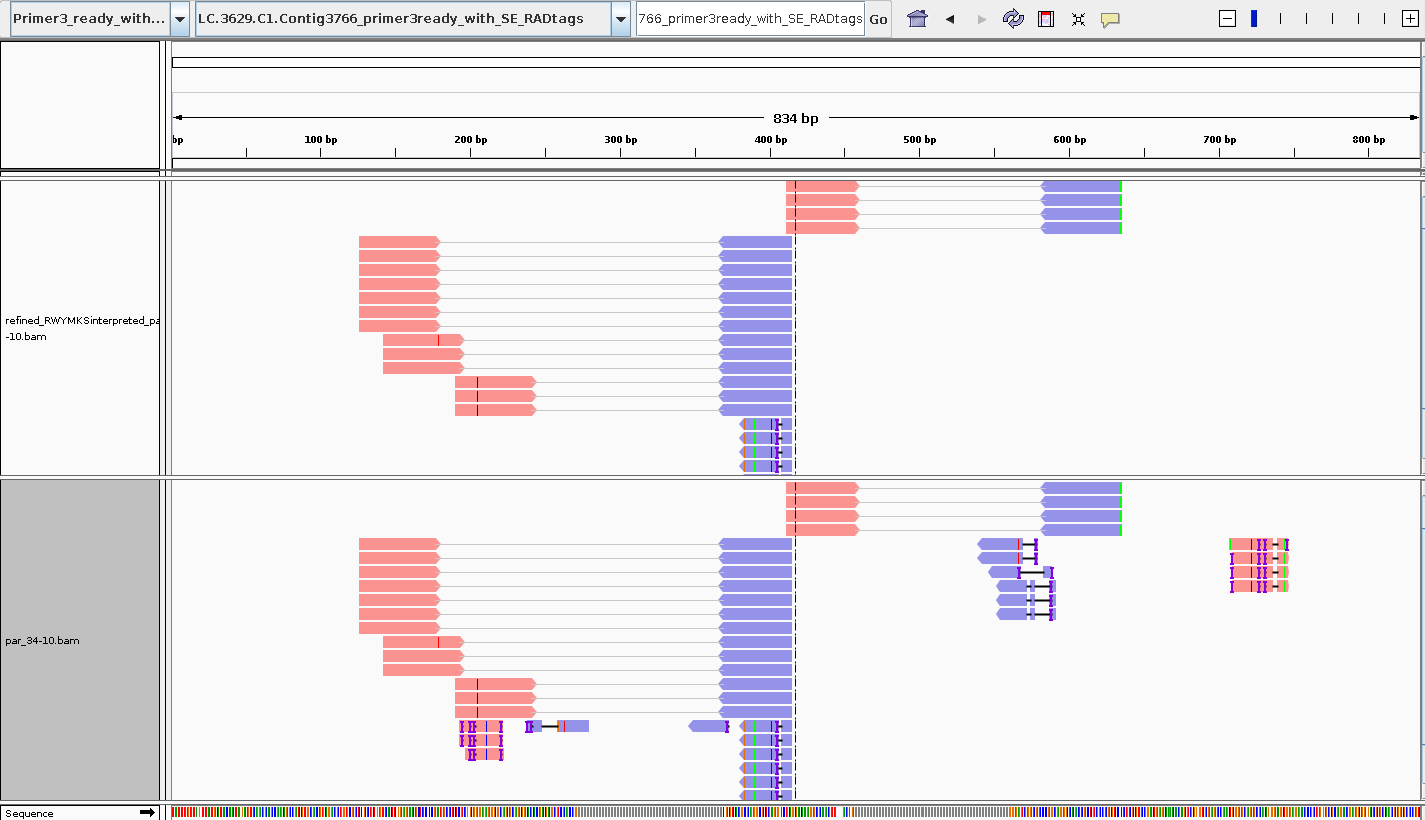
\includegraphics[width=\textwidth]{./figure/stampy_par_34-10_vs_primer3ready_after_coval-refine_igv}
\caption{Read alignment of all standard RAD reads of individual par\_34-10 against one detected linked RADtags sequence in the primer3ready\_with\_RADtags reference. Upper track after \texttt{coval-refine} filtering. Lower track is without \texttt{coval-refine} filtering for comparison.}
\label{coval-refine}
\end{figure}

\roger{\texttt{Coval-refine} by default removes all reads with more than 2 indels, 1 indel and 1 soft-clipped end and 2 soft-clipped ends. I have set the maximum proportion of mismatches to 0.1. The single-end reads are 46 base pairs long and are allowed to have up to 5 mismatches. The 51 base pair long paired-end reads are also allowed up to 5 mismatches. Each indel contributes 1 to the mismatch count.} 
I have turned on sequencing error correction mode with a minimum minor allele  frequency of a putative SNP of 0.1. See \texttt{coval.sh} in the \texttt{mapping\_against\_primer3ready\_seqs} directory. 
\roger{Figure \ref{coval-refine} shows the mapping result after \texttt{coval-refine} treatment for one individual and one reference sequence.}

\roger{By default, \texttt{coval-refine} counts ambiguous positions in the reference as mismatches. I changed \texttt{coval-refine-sam.pl} to take correct account of the dual ambiguity codes RWYMKS.} I created a git repository in "/usr/local/share/Coval/coval-1.4.1" to track my changes to the \texttt{Coval} programmes. See commit messages for the changes I introduced.

\texttt{IGV} allows to load many .bam files into a single track by specifying a .bam.list file containing the path names to the files to load. It can then colour reads by individual ID or by sample/population. This information is taken from the RG:ID and RG:SM tags in the bam files, respectively. I wrote a perl script called \texttt{add\_RG\_tag.pl} that takes a list of sam/bam files and inserts RG tags into their header as well as each SAM record if they are not already present. This allows me now to load the mapped and coval-refined reads of all 36 individuals into \texttt{IGV} and colour reads by individual or by population.

\hypertarget{CCGGT}{
\texttt{find\_linked\_RADtags.pl} did not output any reads from individual with barcode CCGGT for RAD site on \textit{Schistocerce} Contig1776. 
}
However, the "all\_Big\_Data.bam" file (that I ran \texttt{find\_linked\_RADtags.pl} on) does contain reads from this individual that mapped to that contig. Their CIGAR strings all contain multiple indels. 


I did a major revamp of \texttt{find\_linked\_RADtags.pl}. The previous version did not correctly transform the mapping position of reads mapping as reverse complement. Read mappers report the mapping position for the most 5 prime reference position where the (reverse complemented) read maps. If the mapping starts with an insertion, then the mapping position of the first matching base is reported as the mapping position of the read. In order to determine whether a reverse and a forward mapping SE read could come from the same RAD site, the most 3 prime mapping position of the reverse mapping read first needs to be determined. Accounting for the expected overlap of the two reads, the 3 prime mapping position of the reverse read should be equal to the mapping position of the forward mapping read. In order to derive the 3 prime mapping position of reverse mapping reads, the previous version only added the read length to the reported mapping position. This does not lead to the correct result if the read contains indels. The new version of the script instead adds the lengths of matches "M" and deletions "D" reported in the CIGAR string to the reported mapping position in order to derive the 3 prime mapping position of the read.

The previous version also did not ignore SE reads that end or begin with an insertion depending on whether they map as reverse complement or not, respectively. This can lead to spurious detection of RADtag site.   

The new version of \texttt{find\_linked\_RADtags.pl} finds 82 unigene contigs with detected RADtag sites (as compared to 77 with the previous version). The new version toke 22 min to complete on the \texttt{all\_Big\_Data.bam} file, containing the \texttt{stampy} mapped reads of all 36 indidviduals against the \texttt{Schistocerca} transcriptome. The new version of the script finds 14 contigs that the old version could not find, but "misses" 9 contigs from the old version. Of the 18 \textit{Schistocerca} unigenes for which primer3\_ready sequences could be assembled with output from the previous version of \texttt{find\_linked\_RADtags.pl}, 15 are also detected by the new version of \texttt{find\_linked\_RADtags.pl}. I used command \ref{process-subst} to determine which \textit{Schistocerca} unigenes that made it into the 18 primer3\_ready sequences did not get detected by the new version of \texttt{find\_linked\_RADtags.pl}.

\begin{command}
\captionsetup{type=command}
% see \fvset in preamble for general settings of font size and family
\begin{Verbatim} 
grep -vxf <(awk '{print $1}' flR_output_version_2/all_Big_Data_linked_RADtag_contigs.out) \
Primer3_ready_Schisto_unigenes
\end{Verbatim}
\caption{Command that determines the ID of \textit{Schistocerca} unigenes that have been detected by the old version of \texttt{find\_linked\_RADtags.pl} but not with the new version. The command prints out lines from the second file (Primer3\_ready\_Schisto\_unigenes) that have not been matched by the patterns (here: unigene ID's) in the first "file": <(...). I need to provide a file to the "-f" switch of \texttt{grep}, but I only want to present the first column of all\_Big\_Data\_linked\_RADtag\_contigs.out as patterns. So I am using a \href{http://www.vincebuffalo.com/2013/08/08/the-mighty-named-pipe.html}{process substitution} with \texttt{<(...)} instead of an intermediate file.}
\label{process-subst}
\end{command}

\begin{table}[h]
\hspace{20pt}
\begin{tabular}{ll}
\toprule
     1	& LC.1365.C1.Contig1509 \\
     2	& LC.3754.C1.Contig3884 \\
     3	& LC.689.C1.Contig803 \\
\bottomrule
\end{tabular}
\end{table}

The reason why the second version of \texttt{find\_linked\_RADtags.pl} misses these three unigenes is because it trusts that indels placed by the read mapping programme are correct. I am using mapping output from \texttt{stampy}.  Inspecting the .mas MEGA alignment files that I used in order to create primer3\_ready sequences for these three unigenes and looking at the CIGAR strings of SE reads with proper pair flag that mapped to these three unigenes\footnote{these are the reads that \texttt{find\_linked\_RADtags.pl} uses for detection}, it is obvious that ambiguous insertions are the reason. For the first unigene, the forward mapping reads start with an insertion. Such reads are completely ignored by the new version of the script. The other two unigenes have reads mapped that contain an insertion that hides mismatches. The insertions hide 2 or three mismatches. The previous version of \texttt{find\_linked\_RADtags.pl} basically ignored all indels inferred by the read mapping programme. If a read started with an indel it subtracted its length from the reported mapping position and then simply added the read length to reverse mapping reads. So any inferred indels did not affect the detection of RADtag sites. The 14 unigenes that only the new version detected must have been detected by reads containing inferred indels. Otherwise they would have been detected by the previous version already. Given that \texttt{stampy} seems to have a very low penalty for placing indels\footnote{in LC.689.C1.Contig803, a 5 bp insertion hides just two mismatches}, I wonder whether these 14 new unigenes really contain RADtags.

\begin{table}[h]
\centering
\caption{brief description of read alignments to unigenes only detected by the new \texttt{find\_linked\_RADtags.pl}}
\label{extra-unigenes}
\begin{tabular}{ll}
\toprule
LC.3000.C1.Contig3154 & overlapping SE and PE reads that map as proper pairs \\
LC.91.C7.Contig139 &  same as above \\
LC.4313.C1.Contig4431 & many thousand reads mapped, most reads have indels, \\
& many of them 3, RAD site detection due to chance \\
\bottomrule
\end{tabular}
\end{table}

I selected 3 of the 14 extra unigenes detected by the new version of \texttt{find\_linked\_RADtags.pl}, which were given names containing a contig number indicating that they  could be annotated. I checked their alignments in \texttt{IGV}. Table \ref{extra-unigenes} summarizes the alignments. I conclude from this sample that the new version of \texttt{find\_linked\_RADtags.pl} does not detect new genuine RAD sites. I, therefore, have revert back to the previous detection algorithm that ignored indels. However, instead of simply adding the read length to the mapping position of reverse mapping reads, the script now uses the numbers in the CIGAR string and adds the lengths of "M" and "I" to the mapping position. 

\begin{figure}
\centering
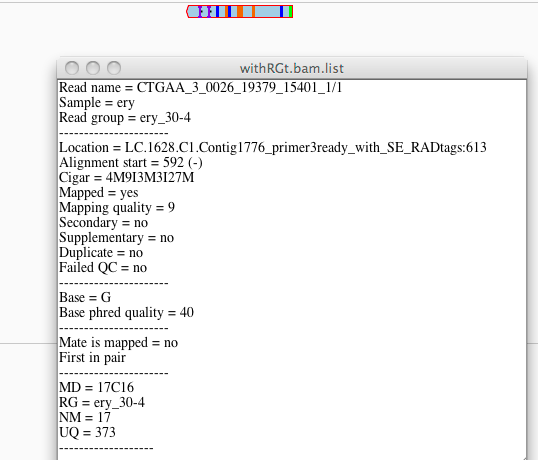
\includegraphics[width=.8\textwidth]{./figure/coval-refine_err-corr}
\caption{A read that is only let through by \texttt{coval refine} if error correction mode is turned on. It looks like only the MD tag is "corrected".}
\label{coval-refine_err-corr}
\end{figure}

The current version of \texttt{find\_linked\_RADtags.pl} will subtract the length of an initial insertion from the mapping position. That is why reads at the bottom of figure \ref{all_SE_pp_on_LC.1628.C1.Contig1776} can detect the RAD site whereas reverse mapping reads that contain insertions after some initial mapping bases (upper half of figure \ref{all_SE_pp_on_LC.1628.C1.Contig1776}) will have an inferred 3 prime mapping position that is beyond the restriction site. So the current version of \texttt{find\_linked\_RADtags.pl} ignores indels unless they occur at the beginning of the aligned read. That is the reason why certain reads map to the "primer3ready\_with\_RADtags" reference that haven't been collected by \texttt{find\_linked\_RADtags.pl}, \hyperlink{CCGGT}{see above}.

\begin{figure}[htb]
\centering
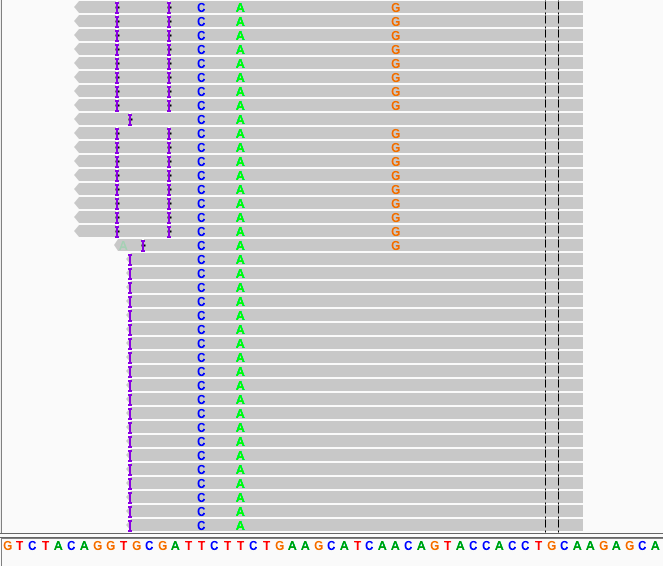
\includegraphics[width=.7\textwidth]{./figure/all_SE_pp_on_LC_1628_C1_Contig1776}
\caption{Snapshot of all SE reads from properly mapped pairs to the \texttt{Schistocerca} contig 1776. }
\label{all_SE_pp_on_LC.1628.C1.Contig1776}
\end{figure}



%%%%%%%%%%%%%%%%%%%%%%%%%%%%%%%%%
\subsection{Evaluation of back mapping}
%%%%%%%%%%%%%%%%%%%%%%%%%%%%%%%%%

I have transferred the .bam files for all 36 individuals to my Mac into the folder \\
\texttt{coval-refined\_RWYMKSinterpreted\_indels\_count\_2\_withRGt}. 
\\
I have also transferred the 18 reference sequences in the file \texttt{Primer3\_ready\_with\_SE\_RADtags.multifas}. I can then open \texttt{IGV} locally on my Mac, load the "genome" and the \texttt{withRGt.bam.list} file. Right-clicking on any read opens a context menu, which allows to select "View as Pairs", "Color Alignments by >  sample" and "Group Alignments by > Read group". This shows the reads of each individual (that has reads mapped the selected reference sequence) in a separate track which is separated by vertical lines from the reads of other individuals (see fig. \ref{IGV-view_group-by-RG}).

\begin{figure}
\centering
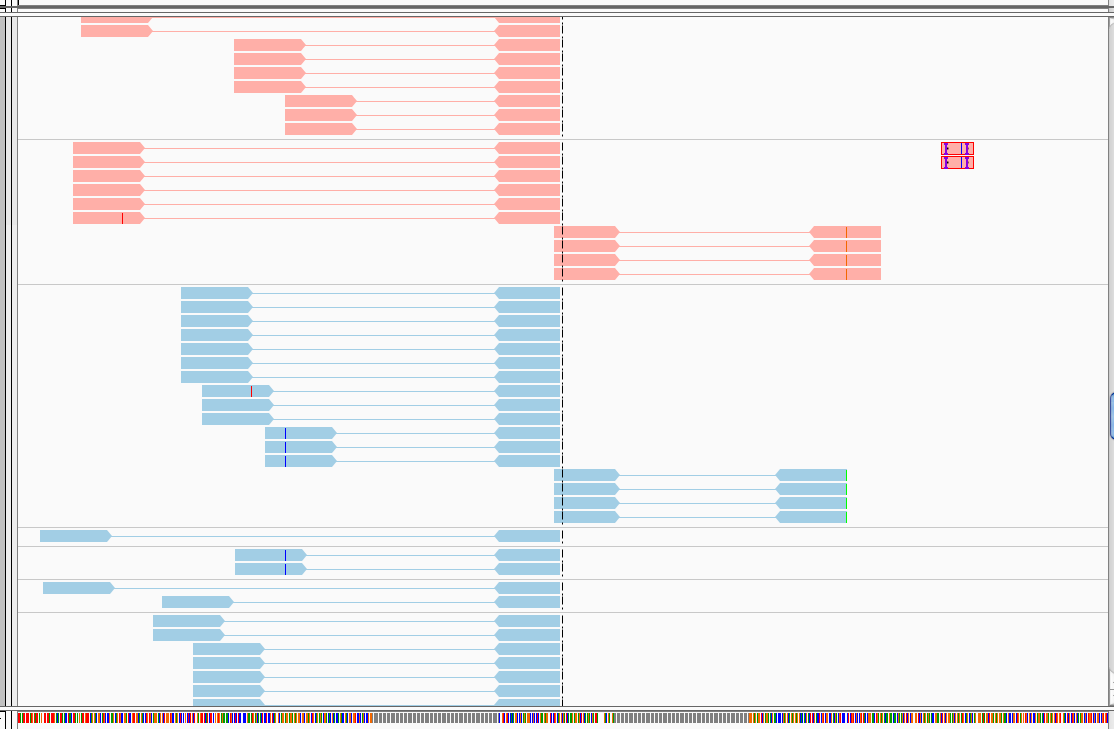
\includegraphics[width=\textwidth]{./figure/IGV-view_group-by-RG}
\caption{Example view of back mapping result on one primer3ready reference sequence. One can see colouring by population. Reads from different individuals are grouped into tracks separated by vertical lines from the reads of other individuals.}
\label{IGV-view_group-by-RG}
\end{figure}

I have had a closer look at the mapping result toward all 18 reference contigs. I have written down a brief descriptions in the \texttt{back-mapping-summary.tab} file, part of which is show in table \ref{back-mapping-summary}. The top 5 reference sequences in table \ref{back-mapping-summary}:

\begin{itemize}
\item do not show very high or very low number of reads mapped
\item do not show large numbers of very divergent reads mostly containing indels
\item do not show other signs of repetitiveness, e. g. SE reads mapping to PE contigs instead of the RAD tags
\end{itemize}

\texttt{LC.3754.C1.Contig3884} only gets reads from \textit{parallelus} (12 individuals) and none from \textit{erythropus}\footnote{except dodgy mappings on the downstream contig}. The assembly of the PE contigs for this unigene was unambiguous. So it is likely that this RAD site does not occur in \textit{erythropus}.


For LC.29.C2.Contig39, only 1 of 17 \textit{erythropus} individuals has a fragment mapped to the downstream side of the RAD site. During the manual merging of \texttt{SSAKE} contigs I noted for this locus that the UPstream PE contig might be duplicated (suspiciously high polymorphism). So one explanation would be that this locus is almost completely absent in \textit{erythropus} and the \textit{erythropus} reads mapping on the upstream side belong to a very similar but different locus.
  
\begin{table}
\centering
\caption{Summary of back mapping to 18 primer3ready with RADtag sequences}
\label{back-mapping-summary}
\begin{tabular}{lccc}
\toprule
Contig name & read number & divergent reads? & repetitive?\\
\midrule
LC.153.C1.Contig213 & - & - & - \\
LC.1628.C1.Contig1776 & - & - & - \\
LC.3629.C1.Contig3766 & - & - & - \\
LC.816.C1.Contig944 & - & - & - \\
LC.3754.C1.Contig3884 & - & - & - \\
LC01053A2H03.f1 & - & div & rep \\
LC03012B1A04.f1 & - & div & rep \\
LC.4254.C1.Contig4373 & high & div & rep \\
LC.637.C2.Contig746 & high & div & rep \\
LC01005A2G05.f1 & high & div & rep \\
LC02008A1C02.f1 & high & div & rep \\
LC03001B1D09.f1 & high & div & rep \\
LC.46.C1.Contig64 & low & - & - \\
LC01010B2D11.f1 & low & - & - \\
LC.1365.C1.Contig1509 & low & - & rep \\
LC.2546.C1.Contig2708 & low & - & rep \\
LC.29.C2.Contig39 & low & - & rep \\
LC.689.C1.Contig803 & low & div & - \\
\bottomrule
\end{tabular}
\end{table}

\roger{For each individual, I counted the fragments (non-PCR duplicates) mapped towards the top four contigs in table \ref{back-mapping-summary} by taking only SE reads from properly mapped pairs and \texttt{uniq}-ing on insert size. Figure \ref{fragments-mapped-per-ind} shows the distribution of these counts over all 36 individuals.}

\roger{None of the 18 loci is a good candidate to test possible variation in digestion. Given the pattern of back mapping at the 4 loci in figure \ref{fragments-mapped-per-ind}, I also now believe that incomplete digestion is unlikely to be the reason for the dominance of singleton loci in the \texttt{stacks} assembly. Even though incomplete digestion cannot be ruled out by this data, a different pattern would be expected if it was common. That is, more individuals would have no fragments mapping while others have many. However, as shown in table \ref{mean_sd_fragNum_per_locus}, the fragment count is generally not very high, indicating that low unique template amount for sequencing prevented any individual from having many fragments mapped.}

\roger{Does the number of reads mapped back from an individual to the primer3ready reference correlate with the total read number of reads from that individual?}

\roger{Yes. Figure \ref{frag_input_corr_fig}, right, shows that fragment count over the four loci (of figure \ref{fragments-mapped-per-ind}) does correlate well with the number of input reads. The left graph in figure \ref{frag_input_corr_fig} also shows that whether an individual misses any fragment from one or more of the four loci correlates with the number of input reads for mapping available for that individual. Both indicates that under-sequencing can partly explain the variation in fragment count among individuals over the four loci. }

\roger{Could this problem be alleviated with sequencing more reads from the same library? I don't think so. It would be very inefficient, since mostly PCR duplicates will be sequenced but few new fragments. Instead, the template amount from each individual for the selective PCR during the library prep needs to be increased. One obvious way would be to increase the total DNA input from each individual, but that reduces the number of individuals that can be pooled during the library prep since the capacity of spin columns and the agarose gel (for size selection) is then reached with fewer individuals. Several libraries would need to be prepared and pooled before selective PCR.
}

\begin{figure}
\begin{knitrout}
\definecolor{shadecolor}{rgb}{0.969, 0.969, 0.969}\color{fgcolor}

{\centering 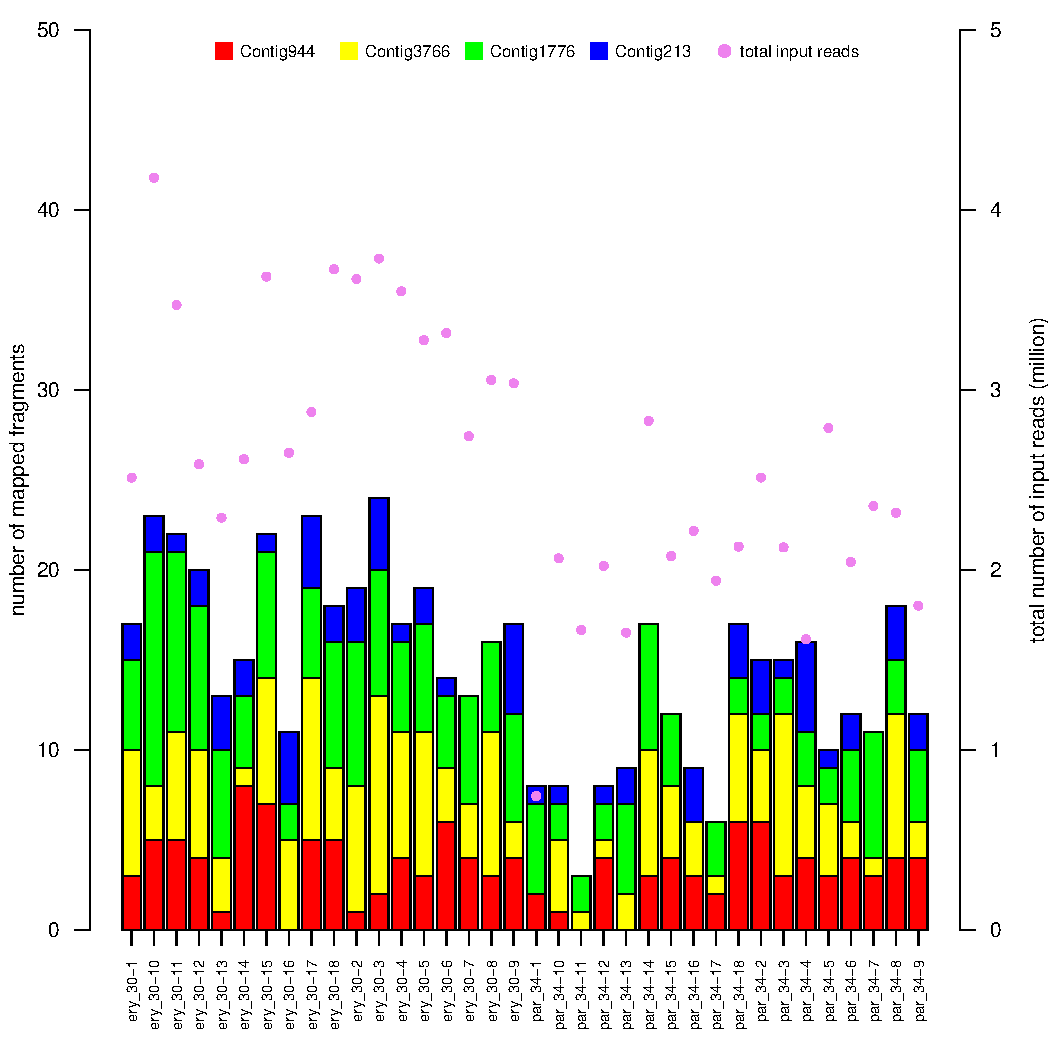
\includegraphics[width=\linewidth]{figure/fragments_mapped_per_ind-1} 

}



\end{knitrout}
\caption{Distribution of RAD fragment numbers mapped to 4 primer3ready reference contigs. A "fragment" is a properly mapped read pair from an individual with a unique insert size. If two read pairs on a RAD site from an individual have the same insert size, they constitute only one fragment, i. e. one read pair is likely to be a PCR duplicate.}
\label{fragments-mapped-per-ind}
\end{figure}


% latex table generated in R 3.0.1 by xtable 1.7-1 package
% Wed Nov 26 12:58:31 2014
\begin{table}[ht]
\centering
\caption{Mean and coefficient of variation of fragment counts for the 4 loci shown in figure \ref{fragments-mapped-per-ind}.} 
\label{mean_sd_fragNum_per_locus}
\begin{tabular}{rrr}
  \hline
 & mean & CV \\ 
  \hline
Contig944 & 3.5 & 0.5 \\ 
  Contig3766 & 4.5 & 0.6 \\ 
  Contig1776 & 4.8 & 0.5 \\ 
  Contig213 & 1.9 & 0.8 \\ 
   \hline
\end{tabular}
\end{table}




\begin{figure}
\begin{knitrout}
\definecolor{shadecolor}{rgb}{0.969, 0.969, 0.969}\color{fgcolor}

{\centering 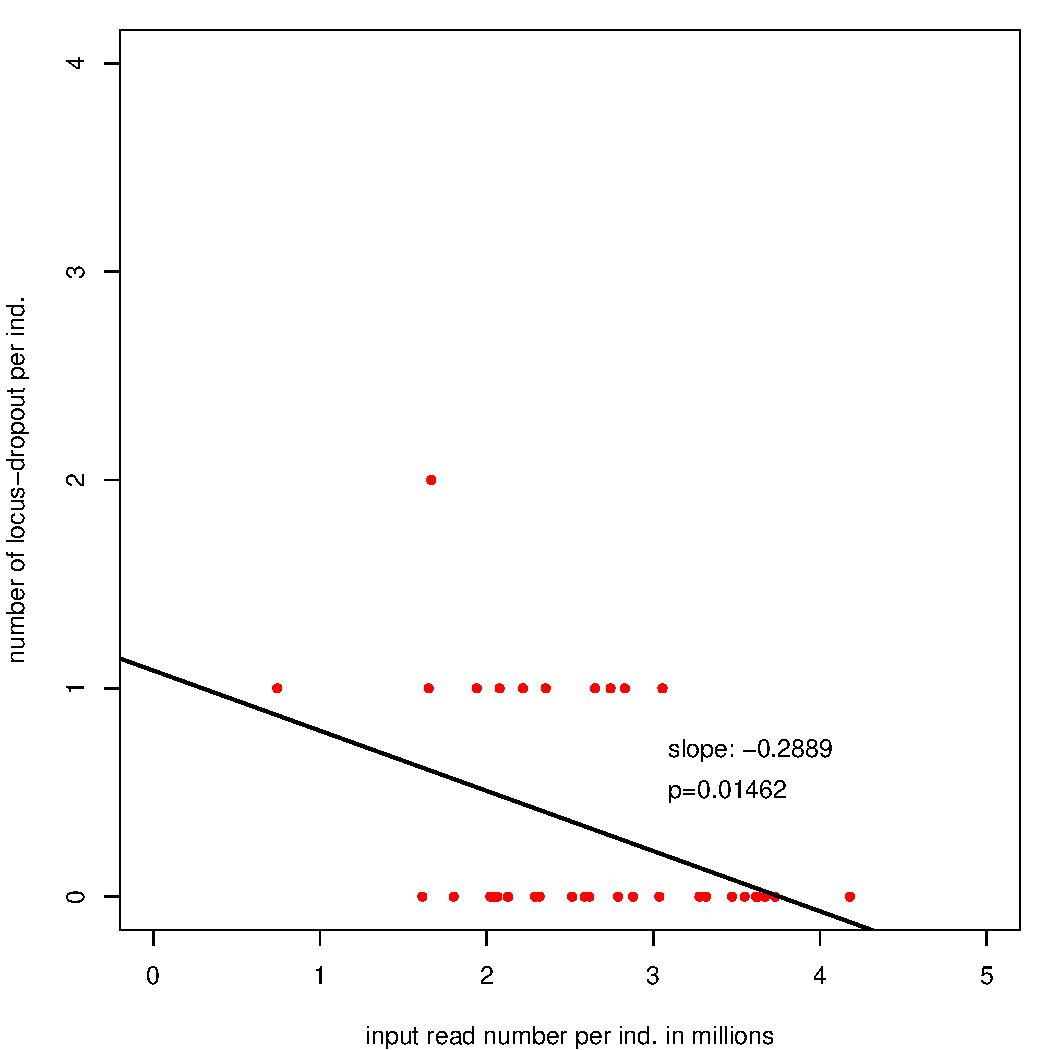
\includegraphics[width=.49\linewidth]{figure/frag_input_corr_fig-1} 
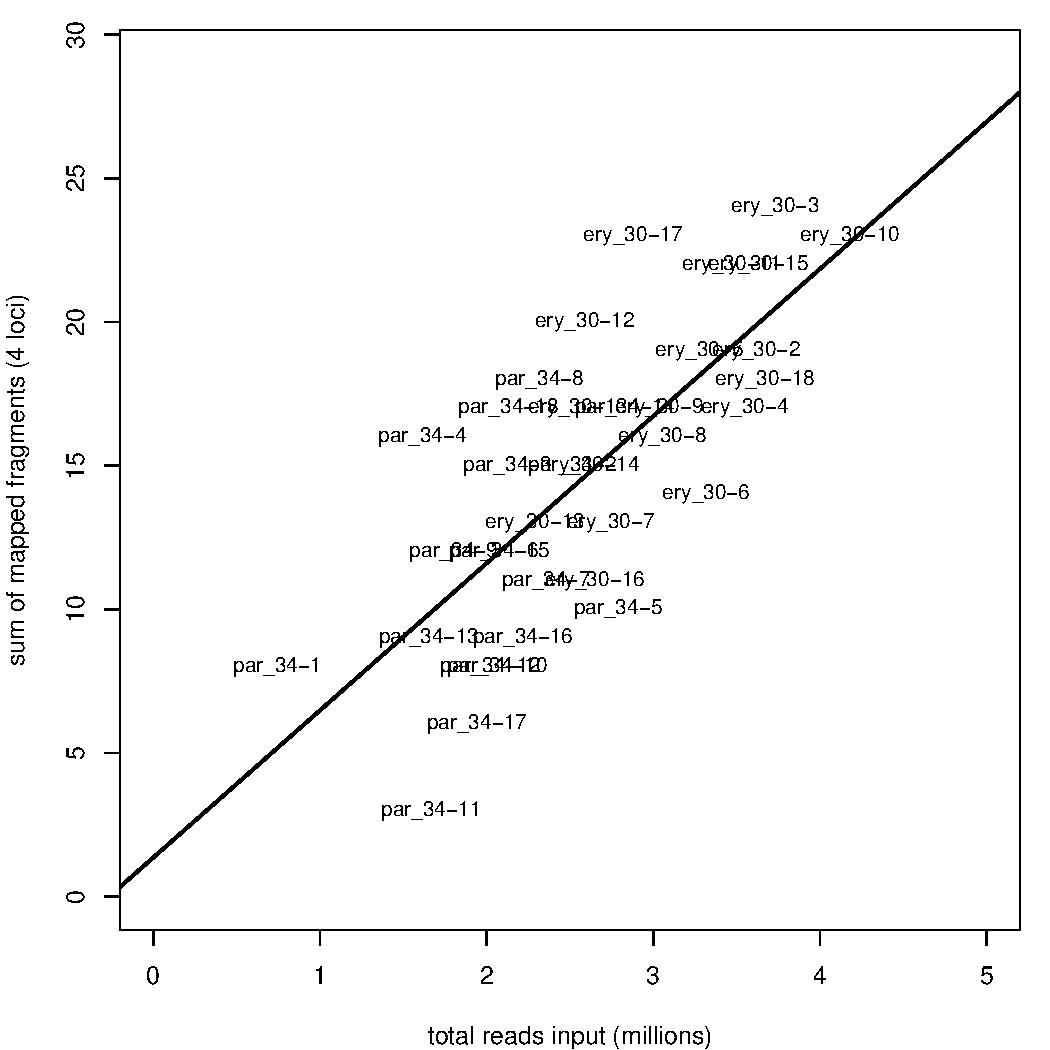
\includegraphics[width=.49\linewidth]{figure/frag_input_corr_fig-2} 

}



\end{knitrout}
\caption{Correlation of locus dropout (left) and fragment counts (right) with number of input reads. Left: Locus dropout is the number of loci (which are the same as in figure \ref{fragments-mapped-per-ind}) for which an individual had no fragment mapped. Right: the sum of mapped fragments over the four loci for each individual versus the number of input reads for the read mapping.}
\label{frag_input_corr_fig}
\end{figure}


\subsubsection{TODO}

\begin{itemize}
\item check other RAD protocols for their template amount per locus per individual for the selective PCR
\item dummy item
\end{itemize}


%%%%%%%%%%%%%%%%%%%%%%%%%%%%%%%%%%
\begin{comment}

\begin{itemize}
\item Why mapping tool test? Shortcomings of stampy, shortcomings of other mapping tool tests
\item Why care about which mapper to use? Does it affect variant calling? structural variation, indels, RNA-seq, Pool-seq are highly affected by read mapping, what false-positive rate for read mapping can be allowed to correctly call indels, etc?
\item simulation of reads from whole reference genome; different simulators, check out dwgsim by Nils Homer
\item high divergence $\leftrightarrow$ low divergence
\item short reads  $\leftrightarrow$ long reads
\item small (low complexity) genome $\leftrightarrow$ large (high complexity) genome
\item runtime
\item mapping whole genome simulated reads against a small subset of the reference
\item real data set with reads from Nicola, capture reads from colour locus
\item real data set, PE read data set from mouse, counting discordantly mapped pairs as the SMALT authors did
\item how is the support of different mapping programmes for long indels?
\end{itemize}


\pagebreak

\texttt{Velvet} is fast, \texttt{VelvetOptimiser} is slow. Write your own Velvetoptimiser script, that just iterates through a kmer range and pick the output containing the longest contig, like the \texttt{SSAKEoptimiser} does.

%%%%%%%%%%%%%%%%%%%%%%%%%%%%%%%%%%
\pagebreak

\begin{itemize}
\item Map assembled contigs against reference
\item try out Columbus extension to \texttt{Velvet}
\item document preparation of the different RAD libraries
\end{itemize}


%%%%%%%%%%%%%%%%%%%%%%
{\color{teal}{

\begin{enumerate}
\item Ana Lopez Sanchez (BMS) uses methylation sensitive restriction enzymes together with PCR to detect methylated DNA in Arabidopsis
\item Is the SbfI digestion complete? Is SbfI digestion variable among individuals due to variation in methylation?
\end{enumerate}

\begin{enumerate}
\item If mapping against a reference is not an option $\Rightarrow$ de novo assembly:
\begin{itemize}
\item digital normalisation
\item Tom Parchman's scripts
\item \texttt{fastqc} provides info on overrepresented kmers in the raw sequence data. I could filter out all reads containing such kmers and thus maybe improve the RAD tag assembly.
\item removing reads which contain over-represented kmers (\texttt{fastqc, windowmasker})
\item \texttt{mcl} clustering as in \texttt{rtd}
\item standard de novo assemblers:
\begin{itemize}
\item IDBA, 
\item ALLPATHS, 
\item velvet, 
\item cortex \citep{Iqbal2012}, 
\item LOCAS, 
\item \href{http://denovoassembler.sourceforge.net/}{Ray},
\item Abyss
\end{itemize}
\end{itemize}
\end{enumerate}
}}
{\color{teal}
Can \texttt{stampy} deal with input sequences containing uncalled bases?
\begin{itemize}
\item MiSeq sequences for a start
\item use reads used for the \texttt{rtd} run, which are only split by barcode, but have fake barcodes inserted at the beginning
\item map stacks consensus tags from the standard RAD library against a Locust transcriptome and look for tags that map to the same restriction site
\end{itemize}

\begin{itemize}
\item maker2
\item allPaths-LG
\item GapCloser
\item REAPR
\item CEGMA
\item UNEAK
\end{itemize}
}

\end{comment}

\pagebreak

%%%%%%%%% -- REFERENCES -- %%%%%%%%%%%%%%%%
%\section{References}
%% References with bibTeX database:

\bibliographystyle{elsarticle-harv}
\bibliography{/Users/Claudius/Documents/MyLiterature/Literature}
%%%%%%%% -- REFERENCES -- %%%%%%%%%%%%%%%%


%%%%%%% -- EXAMPLE FROM TEMPLATE -- %%%%%%%%%%%
\begin{comment}
%You can test if \textbf{knitr} works with this minimal demo. OK, let's
%get started with some boring random numbers:
%
%<<boring-random>>=
%set.seed(1121)
%(x=rnorm(20))
%mean(x);var(x)
%@
%
%The first element of \texttt{x} is x[1]. Boring boxplots
%and histograms recorded by the PDF device:
%
%<<boring-plots, fig.width=4, fig.height=4, out.width='.4\\linewidth'>>=
%## two plots side by side (option fig.show='hold')
%par(mar=c(4,4,.1,.1),cex.lab=.95,cex.axis=.9,mgp=c(2,.7,0),tcl=-.3,las=1)
%boxplot(x)
%hist(x,main='')
%@
%
%Do the above chunks work? You should be able to compile the \TeX{}
%document and get a PDF file like this one: \url{https://bitbucket.org/stat/knitr/downloads/knitr-minimal.pdf}.
%The Rnw source of this document is at \url{https://github.com/yihui/knitr/blob/master/inst/examples/knitr-minimal.Rnw}.
\end{comment}
%%%%%%%%%%%%%%%%%%%%%%%%%%%%%%%%%%%%



\end{document}
